\chapter{Symmetrische Verschlüsselung}
\label{cha:symencryption}
Ein symmetrisches Verschlüsselungsverfahren sichert eine Kommunikation zwischen (typischerweise zwei) Parteien durch einen geheimen Schlüssel, den alle Parteien kennen. Der Schlüssel dient sowohl der Chiffrierung als auch der Dechiffrierung. Er wird keiner bestimmten Partei, sondern einer bestimmten Kommunikationsverbindung zugeordnet. Alle klassischen Verschlüsselungsverfahren sind symmetrisch.

Um eine sichere Kommunikation zu beginnen, müssen sich beide Parteien zuvor auf einen gemeinsamen Schlüssel einigen. Diesen Vorgang nennen wir \emph{Schlüsselaustausch}. Bei \emph{offenen} digitalen Systemen, wie dem Internet, können wir nicht davon ausgehen, dass die Kommunikationspartner schon vorher in Kontakt standen: Prinzipiell kann jeder an einem offenen System teilnehmen und hat Zugriff auf die im System angebotenen Dienste. Daher muss der Schlüsselaustausch innerhalb des Systems selbst erfolgen. Schlüsselaustauschverfahren betrachten wir allerdings erst in Kapitel~\ref{cha:keyexchange} und gehen, der Einfachheit halber, zunächst davon aus, dass beide Kommunikationspartner bereits über einen gemeinsamen geheimen Schlüssel verfügen.

Eine Verschlüsselungsfunktion erwartet in der Regel eine Eingabe fester Länge. Daher wird ein Klartext beliebiger Länge vor der Verarbeitung in eine Folge von Blöcken oder Zeichen fester Länge aufgeteilt, die dann einzeln chiffriert werden. Wird für jeden Block die Verschlüsselungsoperation mit dem selben Schlüssel verwendet, so spricht man von \emph{Blockchiffren}. Diese werden in Kapitel~\ref{sec:blockchiffren} ausführlich behandelt. Als \emph{sequentielle Chiffren} oder \emph{Stromchiffren} bezeichnet man Verschlüsselungsverfahren, bei denen die Klartextzeichen nacheinander mit einem in jedem Schritt variierenden Element eines Schlüsselstroms kombiniert werden.

\section{Stromchiffren}
Wir können einen Klartext $\plaint$ als eine endliche Folge $\plaint = (\plaint_i) = (\plaint_1,\plaint_2,\dots,\plaint_n) $ von Zeichen $\plaint_i$ aus einem Klartextalphabet auffassen. Eine Stromchiffre verschlüsselt einen Klartext, indem sie jedes Klartextzeichen $\plaint_i$ durch ein Chiffratzeichen $\ciphert_i$ aus einem Chiffratalphabet ersetzt. Üblicherweise handelt es sich bei den Klartextzeichen um Bits. 

Um die Bits, die zur Verschlüsselung mit dem Klartext verknüpft werden, zu erzeugen, verfügt eine Stromchiffre über einen internen Zustand $\key^{(i)} \in \{0,1\}^k$, der initial auf den Schlüsselwert $\key$ gesetzt wird und eine Funktion
\begin{align*}
	SC(\key^{(i)}) \in \{0,1\} \times \{0,1\}^k\, ,
\end{align*}
die den Zustand von $\key^{(i)}$ auf $\key^{(i+1)}$ aktualisiert. Der Schlüssel $\key$ ist das Geheimnis, dass sich beide Parteien, das heißt, der Ver- und der Entschlüssler, teilen. Formal ist eine Funktion $G(\key) \coloneqq (b^{(1)},\dots,b^{(n)})$ definiert, die die Folge der Verschlüsselungsbits mit Hilfe von $SC$ aus $\key$ extrahiert:
\begin{align*}
	&\key^{(0)} \coloneqq \key\\
	&\textnormal{Für } i = 0,\dots,n-1\colon (b^{(i+1)},\key^{(i+1)}) \coloneqq SC(\key^{(i)}) 
\end{align*}
$G$ bezeichnen wir auch als Generator. Für das Chiffrat $\ciphert$ gilt dann $\ciphert \coloneqq \plaint \circ G(\key)$, wobei $\circ$ eine binäre Verknüpfung auf Bits ist. Häufig wird hier die logische XOR-Operation, das heißt, die Addition in $\mathbbm{Z}_{2}$, die wir nachfolgend durch $\oplus$ ausdrücken, verwendet. Das Chiffratzeichen $\ciphert_{i}$ ist in diesem Fall durch $\ciphert_{i} \coloneqq \plaint_{i} \oplus b^{(i)}$ gegeben. 

Da Stromchiffren die Chiffratzeichen unabhängig voneinander berechnen, lassen sich solche Verschlüsselungsverfahren effizient in Hardware parallelisieren. Zusätzlich trägt die Verwendung einer binären Operation mit niedriger Komplexität, wie zum Beispiel $\oplus$, zu einer effizienten Ausführung bei.

\begin{figure}[h]
	\centering
	\tikzstyle{every circle node}= [draw]
	\begin{tikzpicture}
	\begin{scope}[>=latex] %for filled arrow tips
	
	%defines
	\pgfmathsetmacro\KXCoord{(0.0)} % K X-Koordinate
	\pgfmathsetmacro\GYCoord{(-1.5)} % G Y-Koordinate
	\pgfmathsetmacro\EncYCoord{(-3.2)} % ENC Y-Koordinate
	
	%draw K_0, SC_Box and connection line
	\node (K) at (\KXCoord,0) {$\key$};
	\node (G) at (\KXCoord, -1.5) [draw,fill=black!15,rectangle, minimum size=20pt] {$G$};
	\draw[->,semithick] (K) -- (G);
	
	%draw XOR operator and conection line SC_Box - XOR
	\node (ENC) at (0,\EncYCoord) [draw,fill=black!15,rectangle, minimum size=20pt] {$\circ$};
	\draw[->, semithick] (ENC) (G) -- (ENC);
	\node (BI) at ({\KXCoord + 0.4}, {\GYCoord - ((\GYCoord - \EncYCoord) * 0.5)}) {$b^{(i)}$};
		
	\node (M) at ({\KXCoord - 2.5}, \EncYCoord) {$\plaint_i$};
	\node (C) at ({\KXCoord + 2.5}, \EncYCoord) {$\ciphert_i$};
	\draw[->,semithick] (M) -- (ENC);
	\draw[->,semithick] (ENC) -- (C);
	
	\end{scope}
	\end{tikzpicture}
	\caption{Prinzip einer Stromchiffre. Der Klartextstrom $(\plaint_1,\plaint_2,\dots,\plaint_n)$ wird mit einem, aus dem Schlüssel $\key$ mit Generator $G$ erzeugten Bitstrom $(b^{(1)}, b^{(2)}, \ldots, b^{(n)})$ durch $\circ$ verknüpft.}
	\label{fig:streamcipher}
\end{figure}

%\begin{figure}[h]
%	\centering
%	\unitlength=1mm
%	\linethickness{0.4pt}
%	\begin{picture}(70,50)
%		\put(5,5){\makebox(0,0)[cc]{$\plaint_i$}}
%		\put(10,5){\vector(1,0){20}}
%		\put(31,2){\framebox(8,6)[cc]{$\enc$}}
%		\put(40,5){\vector(1,0){20}}
%		\put(65,5){\makebox(0,0)[cc]{$\ciphert_i$}}
%		\put(35,20){\vector(0,-1){10}}
%		\put(35.5,13){\makebox(6,6)[cc]{$b^{(i)}$}}
%		\put(32,22){\framebox(6,6)[cc]{$G$}}
%		\put(35,40){\vector(0,-1){10}}
%		\put(35,45){\makebox(0,0)[cc]{$\key$}}
%	\end{picture}
%	\caption{Prinzip einer Stromchiffre. Der Klartextstrom $(\plaint_1,\plaint_2,\dots,\plaint_n)$ wird zeichenweise mit einem, aus dem Schlüssel $\key$ mit
%	Generator $G$ erzeugten Bitstrom $(b^{(1)}, b^{(2)}, \ldots, b^{(n)})$ durch $\enc$ verschlüsselt.}
%	\label{fig:streamcipher}
%\end{figure}

Wir bemerken, dass gleiche Klartextzeichen an verschiedenen Positionen nicht notwendigerweise durch das gleiche Chiffratzeichen codiert werden: Im Allgemeinen folgt für $i \ne j$ aus $\plaint_i = \plaint_j$ also nicht $\ciphert_i = \ciphert_j$. Eine derartige Zeichenersetzung heißt \emph{polyalphabetische Substitution}. An dieser Stelle sei erwähnt, dass eine Stromchiffre nicht auf dem ursprünglichen Alphabet des Klartextes arbeiten muss. Sie verwendet jedoch elementare Einheiten "`kleiner"' Länge, aus denen der Klartext durch Konkatenation aufgebaut werden kann. Solche Einheiten nennen wir im Folgenden Zeichen.
%TODO: Nach unserer Auffassung, ist polyalphabetische Substitution etwas anderes.
%TODO: Auf was bezieht sich der letzte Satz? Eingabe/Ausgabe?

Das klassische Beispiel einer Stromchiffre ist die in Abschnitt~\ref{ssec:vigenere} vorgestellte \emph{Vigenère"=Chiffre}. Im Gegensatz zur Vigenère"=Chiffre bietet eine Stromchiffre, die auf einer wirklich zufälligen Schlüsselfolge basiert, perfekte Geheimhaltung der verschlüsselten Nachricht. Dieses Verfahren heißt \emph{One-Time-Pad} und wird im Abschnitt~\ref{ssec:otp} vorgestellt.

\subsection{Caesar-Chiffre}
Eine der ersten schriftlich belegten Chiffren ist die \emph{Caesar-Chiffre}. Der Name stammt vom römischen Feldherrn Julius Caesar, der nach Aufzeichnungen des römischen Schriftstellers Sueton seine militärische Korrespondenz verschlüsselte, indem er jeden Buchstaben des lateinischen Alphabets zyklisch um 3 nach rechts verschob.
\begin{table}[h]
	\centering
	\setlength{\tabcolsep}{2pt}
	\begin{tabular}{l*{26}{c}}
		Klartextalphabet: &A&B&C&D&E&F&G&H&I&J&K&L&M&N&O&P&Q&R&S&T&U&V&W&X&Y&Z\\
		Geheimtextalphabet: &D&E&F&G&H&I&J&K&L&M&N&O&P&Q&R&S&T&U&V&W&X&Y&Z&A&B&C\\
	\end{tabular}
	\caption{Buchstabensubstitution gemäß der Caesar-Chiffre}
\end{table}

Aus dem Klartext \glqq CHIFFRE\grqq{} wird damit beispielsweise das Chiffrat \glqq FKLIIUH\grqq. Zur Entschlüsselung werden die Buchstaben im Geheimtextalphabet entsprechend um 3 nach links verschoben. Das Problem bei dieser Art von Verschlüsselung ist unmittelbar ersichtlich: Die Methode verändert sich nicht. Daher kann jeder, der einmal erkannt hat, wie Caesar seine Nachrichten verschlüsselte, diese ohne Probleme entschlüsseln. Es gibt keinen Schlüssel und die Sicherheit des Verfahrens hängt allein von der Geheimhaltung der Chiffre ab.

Manchmal wird auch die allgemeine \emph{Verschiebe-Chiffre} als Caesar-Chiffrierung bezeichnet. Bei dieser Chiffre gibt es einen Schlüssel $\key$, der die Anzahl der Stellen angibt, um die zyklisch verschoben wird. Dient das lateinische Alphabet als Grundlage, ist $\key \in \{0,\dots,25\}$. Einen Klartext $\plaint$ der Länge $n$ betrachten wir dementsprechend als Zahlenstrom, der sich ergibt, indem jeder Buchstabe $\plaint_{i}, i \in \{1,\dots,n\}$ aus $\plaint$ auf die Zahl, die der Stelle des Buchstabens im zugrundeliegenden Alphabet entspricht, abgebildet wird. Für das lateinische Alphabet ist der resultierende Zahlenstrom also aus $\{0,\dots,25\}^{n}$. 

Die Chiffratzeichen $\ciphert_{i}, i \in \{1,\dots,n\}$ erhalten wir durch 
\begin{align*}
	\enc(\key, \plaint_i) = \plaint_i + \key \mod 26
\end{align*}
und entschlüsseln gemäß
\begin{align*}
	\dec(\key, \ciphert_i) = \ciphert_i - \key \mod 26\, .
\end{align*}
Da allerdings nur 26 mögliche Schlüssel existieren, ist es selbst ohne Computerunterstützung möglich, jeden Schlüssel auszuprobieren. Ein solcher Angriff wird als \emph{Exhaustive Search} oder \emph{Brute-Force-Angriff} bezeichnet.

%\begin{figure}[h]
%	\centering
%	\unitlength=1mm
%	\linethickness{0.4pt}
%	\begin{picture}(100,30)
%		\put(5,5){\makebox(0,0)[cc]{$\plaint_i$}}
%		\put(10,5){\vector(1,0){20}}
%		\put(32,2){\framebox(35,6)[cc]{$(\plaint_i + \key) \mod 26$}}
%		\put(70,5){\vector(1,0){20}}
%		\put(95,5){\makebox(0,0)[cc]{$\ciphert_i$}}
%		\put(50,20){\vector(0,-1){10}}
%		\put(47,22){\makebox(6,6)[cc]{$\key$}}
%	\end{picture}
%	\caption{Prinzip einer Verschiebe-Chiffre. Der Klartextstrom $(\plaint_1,\plaint_2,\ldots,\plaint_n)$ wird zeichenweise um den Schlüssel $\key \in \{ 1,\ldots,26\}$ verschoben.}
%	\label{fig:caesarcipher}
%\end{figure}

Diese Beobachtung führt zu dem wichtigen Prinzip, dass jedes sichere Verschlüsselungsverfahren einen Schlüsselraum besitzen muss, der nicht durch Exhaustive Search angreifbar ist. Im heutigen Zeitalter, in dem für einen Brute-Force-Angriff ein Netz aus mehreren tausend Computern benutzt werden können, muss der Schlüsselraum groß sein \cite{NIST_800_57, Blaze1996}. Es ist jedoch wichtig zu verstehen, dass das obige Prinzip lediglich eine notwendige und keine hinreichende Bedingung für ein sicheres Verschlüsselungsverfahren darstellt.

Interessanterweise ist eine Variante der Caesar-Verschlüsselung heute weit verbreitet. Sie wird \emph{ROT-13} genannt und führt eine zyklische Verschiebung
um 13, anstatt um 3 Stellen durch. Diese Art der Verschlüsselung bietet zwar keine kryptographische Sicherheit, wird jedoch dazu verwendet, um Spoiler oder Pointen bis zu einer bewussten Entschlüsselung zu verschleiern. Der Vorteil von ROT-13 besteht darin, dass Ver- und
Entschlüsselung exakt die selbe Funktion verwendet, was für eine einfache Implementierung sorgt.

\subsection{Vigenère-Chiffre}
\label{ssec:vigenere}
Eine Weiterentwicklung der Caesar-Chiffre, die mehr Sicherheit bietet, ist die sogenannte \emph{Vigenère-Chiffre}, benannt nach einem Franzosen des
sechzehnten Jahrhunderts, Blaise de Vigenère. Im Gegensatz zur Caesar-Chiffre besteht der Schlüssel $\key = (\key_{1},\key_{2},\dots,\key_{m}) \in \{0,\dots,25\}^{m}$ nicht zwangsläufig aus einem Zeichen, sondern einer Zeichenfolge der Länge $1 \leq m$.
Der Zeichenvorrat ist das lateinische Alphabet mit seinen 26 Buchstaben. Die Verknüpfung der Schlüsselfolge mit der Klartextfolge geschieht durch die zeichenweise Addition modulo~26. Für den Fall, dass die Schlüssellänge kürzer als die Klartextfolge ist, das heißt $m < n$, wird das Schlüsselwort periodisch wiederholt.
\begin{align*}
	\begin{split}
		(\ciphert_{1},\ciphert_{2},\dots,\ciphert_{m},\ciphert_{m+1},\dots) &= (\plaint_{1},\plaint_{2},\dots,\plaint_{m},\plaint_{m+1},\dots)\\ 
		&+ (\key_{1},\key_{2},\dots,\key_{m},\key_{1},\dots) \mod 26
	\end{split}
\end{align*}
Für ein Chiffratzeichen $\ciphert_{i}, i \in \{1,\dots,n\}$ heißt das im Allgemeinen:
\begin{align*}
	\ciphert_{i} \coloneqq \plaint_{i} + \key_{(i-1 \bmod m)+1} \mod 26
\end{align*}

\begin{table}[h]
	\centering
	\setlength{\tabcolsep}{2pt}
	\begin{tabular}{ll}
		Schlüssel: 
		& SICHER
	\end{tabular}
	\begin{tabular}{l*{26}{c}}
		Klartext:
		&A&B&C&D&E&F&G&H&I&J&K&L&M&N&O&P&Q&R&S&T&U&V&W&X&Y&Z\\
		Schlüsselfolge:
		&S&I&C&H&E&R&S&I&C&H&E&R&S&I&C&H&E&R&S&I&C&H&E&R&S&I\\
		Geheimtext:
		&T&K&F&L&J&X&Z&Q&L&R&P&D&F&W&R&X&V&J&L&C&X&D&B&P&R&I\\
	\end{tabular}
	\caption{Beispiel einer Vigenère-Chiffre}
\end{table}

%\begin{figure}[h]
%	\centering
%	\unitlength=1mm
%	\linethickness{0.4pt}
%	\begin{picture}(100,50)
%		\put(5,5){\makebox(0,0)[cc]{$\plaint_i$}}
%		\put(10,5){\vector(1,0){20}}
%		\put(32,2){\framebox(35,6)[cc]{$(\plaint_i + \key'_i) \mod{} 26$}}
%		\put(70,5){\vector(1,0){20}}
%		\put(95,5){\makebox(0,0)[cc]{$\ciphert_i$}}
%		\put(50,20){\vector(0,-1){10}}
%		\put(50,13){\makebox(6,6)[cc]{$\key'_i$}}
%		\put(30,22){\framebox(40,6)[cc]{$\key'_i = \key_{((i - 1) \mod{} l) + 1}$}}
%		\put(50,40){\vector(0,-1){10}}
%		\put(50,45){\makebox(0,0)[cc]{$\key$}}
%	\end{picture}
%	\caption{Prinzip einer Vigen\`ere"=Chiffre. Der Schlüsselstrom $\key_i'$ entsteht durch Wiederholung des Schlüssels $K \coloneqq (\key_{1},\key_{2},\dots,\key_{m})$:
%	$\key'_i = \key_{((i - 1) \;  \mod{}  \; l) + 1}$, wobei $l$ die Länge des Schlüssels $\key$ ist. Der Klartextstrom $(\plaint_1,\plaint_2,\ldots,\plaint_n)$ wird zeichenweise, entsprechend der Verschiebe-Chiffre, mit dem passenden Buchstaben des Schlüsselstroms verschlüsselt.}
%	\label{fig:vigerecipher}
%\end{figure}

%\begin{figure}[h]
%	Ist $\underline k = (k_1,\ldots,k_{l})$ eine Schlüsselfolge der Länge $l$, so ist die Chiffrierabbildung der Vigen\`ere-Chiffre gegeben durch:
%	\begin{equation*}
%		E_{\underline k} : m_1\ldots m_{r} \mapsto t_{k_1}(m_1)\ldots t_{k_{l}}(m_{l})t_{k_1}(m_{l+1})\ldots t_{k_{r\bmod{l}}}(m_{r})
%	\end{equation*}
%	\begin{equation*}
%		\begin{array}{rp{14cm}}
%	    		{\rm mit\colon\ }		& $m_1\ldots m_{r}$ Klartextfolge der Länge $r$ und\\
%							& $t_{k_j}(m_i) := m_i + k_j \bmod{n}$, wobei die Indices von $k$ als die Repräsentanten\\
%							& $1,\dots,l$ der Restklassen modulo $l$ zu verstehen sind.
%		\end{array}
% 	\end{equation*}
% \end{figure}

\begin{figure}[h]
	Für einen Schlüssel der Länge $m$  und einen Klartext der Länge $n$ ist die Chiffrierabbildung der Vigenère-Chiffre gegeben durch:
	\begin{align*}
		\enc_{\key} : (\plaint_1,\ldots,\plaint_{n}) \mapsto (t_{\key_1}(\plaint_1),\ldots,t_{\key_{m}}(\plaint_{m}),t_{\key_1}(\plaint_{m+1})\ldots,t_{\key_{(n-1 \bmod m)+1}}(\plaint_{n}))\, ,
	\end{align*}
	wobei $t_{\key_{j}}(\plaint_{i}) \coloneqq \plaint_{i} + \key_{j} \mod 26$, $j = (i-1 \bmod m)+1$.
\end{figure}
Erst das Wiederholen einer im Verhältnis zum Klartext kurzen Schlüsselfolge ermöglicht die Kryptoanalyse des Vigenère"=Systems.
Der Weg über die Analyse der Häufigkeitsverteilung der Zeichen im Chiffretext (Aufstellen der Histogramme) führt hier nicht zum Ziel, da die Histogramme für
lange Schlüssel verflachen, d.h. sich einander angleichen. Daher ist eine Vigenère"=Chiffre wesentlich sicherer als eine einfache Substitution von
Buchstaben; sie wurde sogar bis Mitte des vorletzten Jahrhunderts für unbrechbar gehalten und als \emph{Le Chiffre indéchiffrable} bezeichnet.
%TODO: {Citation needed}

Allerdings ist das Brechen der Vigenère-Chiffre relativ einfach, sobald man die Länge $m$ des Schlüssels kennt. Die Länge $m$ kann durch einfache Überlegungen bestimmt werden: Man betrachte für $\tau = 1,2,\ldots$ die entsprechenden Geheimtextbuchstaben $t_{\key_j}(\plaint_j),t_{\key_j}(\plaint_{\tau+j}),t_{\key_j}(\plaint_{2 \cdot \tau+j}),\ldots$ und die Gleichung
\begin{equation*}
	S_{\tau}=	\sum_{i=0}^{25} q^2_i \, \text{,}
\end{equation*}
wobei $q_i$ die Anzahl der Vorkommen des i-ten Buchstaben des Alphabets in der Sequenz geteilt durch die Summe aller Buchstaben der Sequenz ist. Sollte für die
Schlüsselänge $l = \tau$ gelten, so wäre zu erwarten, dass $S_{\tau}$ ungefähr den gleichen Wert hat wie unter den Wahrscheinlichkeiten eines
natürlichsprachlichen Textes, da eine Verschiebe-Chiffre die Häufigkeitsverteilung nicht verschleiert. Der Wert der Summe entspräche dann annähernd $0.075$.
Für $l \neq \tau$ ist dagegen zu erwarten, dass alle Buchstaben mit ungefähr gleicher Wahrscheinlichkeit in der Folge $t_{k_j}(m_j),$ $t_{k_j}(m_{\tau+j}),$ $t_{k_j}(m_{2 \cdot \tau+j}),\ldots$ auftreten, also $\forall i\colon~q_i~\approx~\frac{1}{26}$ und somit
\begin{equation*}
	S_{\tau} \approx \sum_{i=0}^{25} (1/26)^2 \approx 0.038 \,\text{.}
\end{equation*}
$S_{\tau}$ unterscheidet sich für $l = \tau$ erkennbar von $l \neq \tau$ und ist der Grund, weshalb diese Methode funktioniert, sofern das Chiffrat eine hinreichende Länge besitzt. Alternativ kann die Länge der Schlüsselfolge mit Hilfe der \emph{Kasiski-Friedmann-Methode} \cite{Kasiski1863} ermittelt werden.

Nun kann das Chiffrat in $l$ unterschiedliche Teilfolgen ($t_{k_j}(m_j),$ $t_{k_j}(m_{l+j}),$ $t_{k_j}(m_{2 \cdot l+j}),\ldots$), $1 \leq j \leq l$ aufgespalten werden, wobei die Verschlüsselung der einzelnen Folgen einer Verschiebe-Chiffre entspricht, die leicht mit Hilfe von Histogrammen gebrochen werden kann.

\subsection{One-Time-Pad}
\label{ssec:otp}
Das \emph{One-Time-Pad} ist eine Stromchiffre mit folgenden Eigenschaften:
\begin{itemize}
	\item Der zur Verschlüsselung verwendete Schlüssel $\key$ besitzt die gleiche Länge $n$ wie der Klartext $\plaint$.
	\item Der Schlüssel wird zufällig gleichverteilt aus dem Schlüsselraum $K \in \{0,1\}^{n}$ ausgewählt. Jeder Schlüssel wird also mit einer Wahrscheinlichkeit von $\frac{1}{2^{n}}$ gewählt.
 	\item Zur Verschlüsselung wird der Klartext und der Schlüssel bitweise mit XOR verknüpft: $\forall i \in \{1,\dots,n\}\colon \ciphert_i = \plaint_i\oplus\key_i$.
 	\item Zur Entschlüsselung wird das Chiffrat und der Schlüssel bitweise mit XOR verknüpft: $\forall i \in \{1,\dots,n\}\colon \plaint_i = \ciphert_i\oplus\key_i$.
  	\item Der Schlüssel darf weder vollständig noch teilweise wiederverwendet werden.
\end{itemize}
Bei Einhaltung aller aufgelisteten Punkte bietet das One-Time-Pad perfekte Geheimhaltung, da, gegeben ein Chiffrat $\ciphert$, jede Nachricht $\{0,1\}^{n}$ gleich wahrscheinlich ist und, da Schlüssel nicht mehrfach verwendet werden, keine Verknüpfung mehrerer Klartexte berechnet werden kann. Natürlich ist zu beachten, dass ein Angreifer, der zumindest den Kontext, indem die Nachrichtenübertragung stattfindet, kennt, sinnvolle von sinnfreien Nachrichten unterscheiden kann.

\begin{beispiel}
\label{ssec:otp:ex:prob}
	Alice möchte Bob unter perfekter Geheimhaltung mitteilen, an welcher Universität sie ihr Studium beginnen möchte. Als Verschlüsselungsverfahren wählen sie das One-Time-Pad. Die Wahl von Alice ist auf das \emph{KIT} gefallen. Binär codiert\footnote{Diese Codierung entspricht dem \emph{8-BIT UCS Transformation Format}, kurz UTF-8.} entspricht das Akronym der Bitfolge $01001011\ 01001001\ 01010100$. Alice wählt zufällig gleichverteilt einen Schlüssel und erhält $K = 00111110\ 01001100\ 10011010$.
	\begin{table}[h]
		\centering
		\setlength{\tabcolsep}{2pt}
		\begin{tabular}{l *{8}{>{$}c<{$}} c *{8}{>{$}c<{$}} c *{8}{>{$}c<{$}}}
			Klartext:
			&0&1&0&0&1&0&1&1&&0&1&0&0&1&0&0&1&&0&1&0&1&0&1&0&0\\
			Schlüssel:
			&0&0&1&1&1&1&1&0&&0&1&0&0&1&1&0&0&&1&0&0&1&1&0&1&0\\
			Geheimtext:
			&0&1&1&1&0&1&0&1&&0&0&0&0&0&1&0&1&&1&1&0&0&1&1&1&0\\
		\end{tabular}
	\end{table}
	
	Ausgehend von dem Chiffrat ist es möglich, einen Schlüssel zu finden, so dass der korrespondierende Klartext ein Akronym einer anderen Universität, wie zum Beispiel \emph{MIT}, ist.
	\begin{table}[h]
		\centering
		\setlength{\tabcolsep}{2pt}
		\begin{tabular}{l *{8}{>{$}c<{$}} c *{8}{>{$}c<{$}} c *{8}{>{$}c<{$}}}
			Geheimtext:
			&0&1&1&1&0&1&0&1&&0&0&0&0&0&1&0&1&&1&1&0&0&1&1&1&0\\
			Schlüssel:
			&0&0&1&1&1&{\color{red} 0}&{\color{red} 0}&0&&0&1&0&0&1&1&0&0&&1&0&0&1&1&0&1&0\\
			Klartext:
			&0&1&0&0&1&1&0&1&&0&0&0&0&0&1&0&1&&1&1&0&0&1&1&1&0\\
		\end{tabular}
	\end{table}
	
	Wir sehen, dass in der gleichen Codierung zwei gekippte Schlüsselbits dem Chiffrat anstelle \emph{KIT} die Buchstaben \emph{MIT} als Klartext zuordnen. Da der Schlüssel zufällig gleichverteilt gezogen wird, ist jeder Schlüssel und somit auch jeder Klartext gleich wahrscheinlich.
\end{beispiel}
%\begin{figure}[h]
%	\centering
%	\unitlength=1mm
%	\linethickness{0.4pt}
%	\begin{picture}(70,30)
%		\put(5,5){\makebox(0,0)[cc]{$\plaint_i$}}
%		\put(10,5){\vector(1,0){20}}
%		\put(35,5){\circle{6}}
%		\put(32,5){\line(1,0){6}}
%		\put(35,2){\line(0,1){6}}
%		\put(40,5){\vector(1,0){20}}
%		\put(65,5){\makebox(0,0)[cc]{$\ciphert_i$}}
%		\put(35,20){\vector(0,-1){10}}
%		\put(32,22){\makebox(6,6)[cc]{$\key_i$}}
%	\end{picture}
%	\caption{Prinzip eines One-Time-Pads. Der Klartextstrom $(\plaint_1,\plaint_2,\ldots,\plaint_n)$ wird zeichenweise mit den Schlüsselstrom $(\key_1, \key_2, \ldots, \key_n)$ binär addiert. Man spricht auch von einer XOR-Verknüpfung.}
%	\label{fig:OTP}
%\end{figure}

Neben dem Vorteil perfekter Geheimhaltung hat das One-Time-Pad auch einige schwerwiegende Nachteile. Ein elementarer Nachteil besteht darin, dass die Schlüssellänge der Länge des Klartexts entsprechen muss und so die zu übermittelnde Datenmenge verdoppelt wird. Dementsprechend schwer gestaltet sich die Übertragung des Schlüsselmaterials, die, um die Eigenschaft perfekter Geheimhaltung nicht zu verletzen, physisch geschehen muss.\footnote{Zur Zeit des Kalten Krieges gab es eine ständig bestehende telegrafische Verbindung zwischen Washington D.C. und Moskau -- genannt \emph{Heißer Draht} oder \emph{Rotes Telefon} --, die mit Hilfe des One-Time-Pads gesichert wurde. Das notwendige Schlüsselmaterial wurde der Gegenpartei in Code-Büchern übergeben.}
Ein weiteres Argument, dass gegen die Verwendung des One-Time-Pads spricht ist, dass für jede Nachrichtenübertragung ein neuer Schlüssel gewählt werden muss, da andernfalls die Eigenschaft der perfekten Geheimhaltung verloren geht. Das lässt sich formal folgendermassen veranschaulichen. Seien $\plaint_{1}, \plaint_{2}$ zwei Klartexte gleicher Länge, die mit Hilfe des One-Time-Pads und dem Schlüssel $\key$ zur Nachrichtenübertragung verschlüsselt werden. Ein Angreifer, der den Kanal abhört und in Besitz der Chiffrate $\ciphert_{1} = \plaint_{1} \oplus \key$ und $\ciphert_{2} = \plaint_{2} \oplus \key$ gelangt, berechnet
\begin{align*}
	\ciphert_{1} \oplus \ciphert_{2} = \plaint_{1} \oplus \key \oplus \key \oplus \plaint_{2} = \plaint_{1} \oplus \plaint_{2}
\end{align*}
und erhält damit im Allgemeinen nicht-triviale Informationen. Ist beispielsweise $M_{1} = 00\dots00$ liefert die Verknüpfung der beiden Geheimtexte den Klartext $M_{2}$. 

Ebenso nachteilig ist, dass das One-Time-Pad bei korrekter Verwendung zwar gegen Angreifer, die die Nachricht lesen möchten, schützt, jedoch nicht gegen Angreifer, die die Nachricht durch Kippen von Bits des Geheimtexts verändern. So könnte ein Angreifer gemäß Beispiel~\ref{ssec:otp:ex:prob} unerkannt zwei Bits des Chiffrats kippen, so dass Bob beim Entschlüsseln auf einen falschen Klartext stößt, nämlich MIT. Gezielte sinnhafte Änderungen des zugrundeliegenden Klartextes sind ohne Schlüsselkenntnis jedoch schwer. 

Die obigen Gründe machen die Verwendung des One-Time-Pad unhandlich, weswegen es nur selten eingesetzt wird. Moderne Stromschiffren funktionieren prinzipiell wie das One-Time-Pad, benutzen jedoch Pseudozufallszahlengeneratoren, die aus einer kurzen Sequenz, genannt \emph{Seed}, den schlussendlich verwendeten Schlüssel als Folge von Pseudozufallszahlen erzeugen.

\subsection{Stromchiffren mit Pseudozufallszahlen}
\label{ssec:stromchiffrenpseudozufall}
Wir wissen bereits, dass die Zufallsfolge, die dem One-Time-Pad als Schlüssel dient, mindestens so lang sein muss, wie die zu verschlüsselnde Nachricht $\plaint$ und nur ein einziges Mal verwendet werden darf. Hieraus folgt, dass dieses Verfahren einen extrem hohen Aufwand für die sichere Schlüsselverteilung erfordert und aus diesem Grund für die meisten Anwendungen nicht praktikabel ist.

\tikzset{XOR/.style={fill=black!15,draw,minimum size=13pt,circle,append after command={
			[shorten >=\pgflinewidth, shorten <=\pgflinewidth,]
			(\tikzlastnode.north) edge (\tikzlastnode.south)
			(\tikzlastnode.east) edge (\tikzlastnode.west)
		}
	}
}

\begin{figure}[h]
	\centering
	\tikzstyle{sc}=[draw,fill=black!15,rectangle,minimum size=20pt,inner sep=0pt]
	\tikzstyle{every circle node}= [draw]
	\begin{tikzpicture}
	\begin{scope}[>=latex] %for filled arrow tips
	
	%defines
	\pgfmathsetmacro\KZeroXCoord{(0.0)} % K^(0) X-Koordinate
	\pgfmathsetmacro\XorYCoord{(-3.0)} % XOR Y-Koordinate
	\pgfmathsetmacro\PYCoord{(-0.75)} % Verbindungspunkt Y-Koordinate
	%\pgfmathsetmacro\minBoxHeight{(0.6)} // 0.5 old
	
	%draw K_0, SC_Box and connection line
	\node (K0) at (\KZeroXCoord,0) {$\key^{(0)}$};
	\node (SC)[sc] at (\KZeroXCoord, -1.5) {$SC$};
	\draw[->,semithick] (K0) -- (SC);
	\node (p1)[circle, fill, inner sep=0cm, minimum size=0.12cm] at (\KZeroXCoord, \PYCoord) {};
	
	%draw XOR operator and conection line SC_Box - XOR
	\node (XOR)[XOR] at (0,\XorYCoord) {};
	\draw[->,semithick] ($(SC) + (0.18, -0.36)$) |- (\KZeroXCoord, -2.25) -- (XOR);
	\node (BI) at ({\KZeroXCoord + 0.18 + 0.4}, -2.25) {$b^{(i)}$};
	
	%draw connection line from SC to connection point p1
	\draw[-,semithick] ($(SC) + (-0.18, -0.36)$) -- (-0.18, -2) -- (-0.5, -2) -- (-0.5, \PYCoord) -- (p1);
	\node (KJ) at (-1.0, {\PYCoord + ((-2 - \PYCoord) * 0.5)}) {$\key^{(j)}$};
	
	
	\node (M) at ({\KZeroXCoord - 2.5}, \XorYCoord) {$\plaint_i$};
	\node (C) at ({\KZeroXCoord + 2.5}, \XorYCoord) {$\ciphert_i$};
	\draw[->,semithick] (M) -- (XOR);
	\draw[->,semithick] (XOR) -- (C);
	
	\end{scope}
	\end{tikzpicture}
	\caption{Prinzip einer Stromchiffre mit Pseudozufall. Der Klartextstrom wird zeichenweise mit einem aus dem Seed $\key^{(0)}$ generierten pseudozufälligen Schlüsselstrom verschlüsselt. Die Entschlüsselung funktioniert analog dazu, das heißt, es wird dieselbe Seed und Funktion $SC$ verwendet. Beachte auch, dass $SC$ nicht in jedem Iterationsschritt ein Verschlüsselungsbit $b^{(i)}$ erzeugen muss, weshalb die Zählvariablen $i$ und $j$ nicht synchron sein müssen.}
	\label{fig:pseudorandomstreamcipher}
\end{figure}

%\begin{figure}[h]
%	\centering
%	\unitlength=1mm
%	\linethickness{0.4pt}
%	\hspace{-3 cm}
%	\begin{picture}(100,50)
%	
%		%Baseline m -> \oplus -> c -> \oplus -> m
%
%		\put(5,5){\makebox(0,0)[cc]{$\plaint_i$}}
%		\put(10,5){\vector(1,0){20}}
%		\put(35,5){\circle{6}}
%		\put(32,5){\line(1,0){6}}
%		\put(35,2){\line(0,1){6}}
%		\put(40,5){\vector(1,0){20}}
%		\put(65,5){\makebox(0,0)[cc]{$\ciphert_i$}}
%		\put(70,5){\vector(1,0){20}}
%		\put(95,5){\circle{6}}
%		\put(92,5){\line(1,0){6}}
%		\put(95,2){\line(0,1){6}}
%		\put(100,5){\vector(1,0){20}}
%		\put(125,5){\makebox(0,0)[cc]{$\plaint_i$}}
%
%		%Encryption
%
%		\put(35,20){\vector(0,-1){10}}
%		\put(35,13){\makebox(6,6)[cc]{$\key'_i$}}
%		\put(27.5,22){\framebox(10,6)[cc]{$SC$}}
%		\put(35,40){\vector(0,-1){10}}
%		\put(35,42){\makebox(0,0)[cc]{$\key_0$}}
%		\put(35,46){\makebox(0,0)[cc]{(\emph{Seed})}}
%		\put(30,20){\line(0,-1){5}}
%		\put(30,15){\line(-1,0){10}}
%		\put(20,15){\line(0,1){20}}
%		\put(20,35){\line(1,0){10}}
%		\put(30,35){\vector(0,-1){5}}
%		\put(25,37.5){\makebox(0,0)[cc]{$\key_{n+1}$}}
%
%		%Decryption
%
%		\put(95,20){\vector(0,-1){10}}
%		\put(95,13){\makebox(6,6)[cc]{$\key'_i$}}
%		\put(87.5,22){\framebox(10,6)[cc]{$SC$}}
%		\put(95,40){\vector(0,-1){10}}
%		\put(95,42){\makebox(0,0)[cc]{$\key_0$}}
%		\put(95,46){\makebox(0,0)[cc]{(\emph{Seed})}}
%		\put(90,20){\line(0,-1){5}}
%		\put(90,15){\line(-1,0){10}}
%		\put(80,15){\line(0,1){20}}
%		\put(80,35){\line(1,0){10}}
%		\put(90,35){\vector(0,-1){5}}
%		\put(85,37.5){\makebox(0,0)[cc]{$\key_{n+1}$}}
%	\end{picture}
%	\caption{Prinzip einer Stromchiffre mit Pseudozufall. Der Klartextstrom wird zeichenweise mit einem aus dem Seed $\key_0$ generierten pseudozufälligen Schlüsselstrom ver- und entschlüsselt. Wichtig ist, dass sowohl bei der Ver-, als auch bei der Entschlüsselung derselbe Seed und dieselbe Funktion $SC$ verwendet wird. Nennenswert ist außerdem, dass die Funktion $SC$ nicht in jedem Iterationsschritt ein Schlüsselbit erzeugen muss, weshalb die Zählvariablen $i$ und $n$ nicht synchron sein müssen.}
%	\label{fig:pseudorandomstreamcipher}
%\end{figure}

Es liegt nahe, die genannte Schwierigkeit zu umgehen, indem man nach dem Vorbild des One-Time-Pad Stromchiffren konstruiert, die statt einer echten Zufallsfolge sogenannte \emph{Pseudozufallsfolgen} verwenden. Unter einer Pseudozufallsfolge versteht man eine Folge von Zeichen, die mittels eines deterministischen Prozesses aus einem relativ kurzen Initialisierungswert, dem Seed, erzeugt wird und gewisse Eigenschaften einer echt zufälligen Folge aufweist. Verfügen beide Kommunikationspartner über identische Generatoren, muss lediglich der Initialwert und die gewählte Parametrisierung des Generators als Schlüssel verteilt werden. Die eigentliche Schlüsselfolge kann dann an beiden Enden des Kanals erzeugt werden.

%Ich bin mir nicht ganz sicher, was mit diesem Abschnitt ausgesagt werden soll. Insbesondere mit dem zweiten Satz.%
Eine Voraussetzung der Konstruktion ist offensichtlich, dass der Pseudozufallsgenerator effizient berechenbar sein muss. Außerdem soll auf den Umstand hingewiesen werden, dass es sich bei der Schlüsselfolge nicht um den Schlüssel des Verfahrens handelt, da die Folge ein Menge von internen Werten des Algorithmus ist. Abbildung~\ref{fig:pseudorandomstreamcipher} zeigt den prinzipiellen Aufbau einer derartigen Stromchiffre.

\subsubsection{Linear Feedback Shift Register}
Eine historisch interessante, aber unsichere Möglichkeit der Implementierung einer Stromchiffre mit Pseudozufall bieten \emph{Linear Feedback Shift
Register} (LFSR). Bei einem LFSR wird der Schlüssel $\key = (\key_{1},\dots,\key_{k})$ zunächst bitweise in Speicherzellen $R_{1},\dots,R_{k}$ angeordnet,
die in jedem Schritt den Zustand beschreiben.
\[    
\begin{tabular}{lc | *{4}{>{\centering}p{0.8cm}|} c}
	\cline{3-6}
	Initialzustand $\key^{(0)}$: && $\key_1$ & $\key_2$ & \dots & $\key_k$ \tabularnewline
	\cline{3-6}
\end{tabular}
\]
Für die Aktualisierung eines Zustandes von $\key^{(i)}$ auf $\key^{(i+1)}$ wird ein Bit 
\begin{align*}
	\key_{k+i+1} \coloneqq \sum^{k}_{j=1} \alpha_{j} \cdot K_{i+j} \mod 2
\end{align*}
berechnet, wobei $\alpha_{i} \in \{0,1\}, i \in \{1,\dots,k\}$ speicherzellenspezifische Koeffizienten sind. Als Verschlüsselungsbit $b^{(i+1)}$ wird das in $R_{1}$ gespeicherte Bit $\key_{i+1}$ ausgegeben. Die verbleibenden Bits $\key_{i+2},\dots,\key_{i+k}$ werden in die jeweils niedriger indexierte Speicherzelle \emph{geschoben}, das heißt $R_{i} = R_{i+1}$. Schlussendlich wird das neu berechnete Bit in die höchstindexierte Speicherzelle geschrieben: $R_{k} = \key_{k+i+1}$.

Für den Übergang aus dem Initialzustand $\key^{(0)}$ zu $\key^{(1)}$ ergibt sich beispielhaft folgendes Schema:

\[
\begin{tabular}{lc | *{4}{>{\centering}p{0.8cm}|} c}
    \cline{3-6}
    $K^{(0)}$: && \(\key_1\) & \(\key_2\) & \dots & \(\key_{k}\) & \\
    \cline{3-6}
    \multicolumn{1}{c}{} &
    \multicolumn{1}{c}{} &
    \multicolumn{1}{c}{\(\downarrow\cdot\alpha_1\)} &
    \multicolumn{1}{c}{\(\downarrow\cdot\alpha_2\)} &
    \multicolumn{1}{c}{\(\ldots\)} &
    \multicolumn{1}{c}{\(\downarrow\cdot\alpha_k\)} & \\
    \multicolumn{1}{c}{} &
    \multicolumn{1}{c}{} &
    \multicolumn{5}{c}{\(\xlongrightarrow{\qquad\qquad\qquad\qquad\qquad\qquad}\ \key_{k+1}:=\sum_{j=1}^{k}\alpha_{j}\key_{j} \mod 2\)}
\end{tabular}
\]

\[
\begin{tabular}{lc | *{4}{>{\centering}p{0.8cm}|} c}
    \cline{3-6}
    $K^{(1)}$: && $\key_{2}$ & \dots & $\key_{k}$ & $\key_{k+1}$ & \\
    \cline{3-6}
    \multicolumn{1}{c}{} &
    \multicolumn{1}{c}{} &
    \multicolumn{1}{c}{\hphantom{\(\downarrow\cdot\alpha_1\)}} &
    \multicolumn{1}{c}{\hphantom{\(\downarrow\cdot\alpha_2\)}} &
    \multicolumn{1}{c}{\hphantom{\(\ldots\)}} &
    \multicolumn{1}{c}{\hphantom{\(\downarrow\cdot\alpha_k\)}} & \\
    \multicolumn{1}{c}{} &
    \multicolumn{1}{c}{} &
    \multicolumn{5}{c}{\hphantom{\(\xlongrightarrow{\qquad\qquad\qquad\qquad\qquad\qquad}\ \key_{k+1}:=\sum_{j=1}^{k}\alpha_{j}\key_{j} \mod 2\)}}
\end{tabular}
\]
%\begin{figure}[h]
%	\centering
%	\unitlength=1mm
%	\linethickness{0.4pt}
%	\hspace{-3 cm}
%	\begin{picture}(100,40)
%		\put(0,35){\makebox(20,5)[cc]{Initialwert}}
%		\put(20,35){\framebox(10,5)[cc]{$K_0$}}
%		\put(30,35){\framebox(10,5)[cc]{$K_1$}}
%		\put(40,35){\framebox(10,5)[cc]{$\ldots$}}
%		\put(50,35){\framebox(10,5)[cc]{$K_{n-1}$}}
%		\put(60,35){\framebox(10,5)[cc]{$K_n$}}
%		\put(20,30){\makebox(10,5)[cc]{$\cdot \alpha_0$}}
%		\put(30,30){\makebox(10,5)[cc]{$\cdot \alpha_1$}}
%		\put(40,30){\makebox(10,5)[cc]{\ldots}}
%		\put(50,30){\makebox(10,5)[cc]{$\cdot \alpha_{n-1}$}}
%		\put(60,30){\makebox(10,5)[cc]{$\cdot \alpha_n$}}
%		\put(20,30){\vector(1,0){50}}
%		\put(82.5,27.5){\makebox(20,5)[cc]{$z = \sum\nolimits^n_{i=0} \alpha_i \cdot K_i$ mod 2}}
%		\put(0,10){\makebox(20,5)[cc]{Zustand $k_1$}}
%		\put(20,10){\framebox(10,5)[cc]{$K_1$}}
%		\put(30,10){\framebox(10,5)[cc]{$K_2$}}
%		\put(40,10){\framebox(10,5)[cc]{$\ldots$}}
%		\put(50,10){\framebox(10,5)[cc]{$K_n$}}
%		\put(60,10){\framebox(10,5)[cc]{$z$}}
%		\put(0,6.5){\vector(1,0){10}}
%		\put(27,4){\makebox(10,5)[cc]{Schlüsselstrom $out_1 = K_0$}}
%	\end{picture}
%	\caption{Prinzip von \emph{Linear Feedback Shift Registern}. In jedem Schritt wird $z$ aus den in den Registern vorhandenen Schlüsselbits und den Konstanten $\alpha_i$ berechnet. $z$ ersetzt dann das Schlüsselbit $\key_n$, welches an Stelle von $\key_{n-1}$ rückt. $\key_{n-1}$ selbst rückt wiederum an Stelle von $\key_{n-2}$ usw. Schließlich wird $\key_0$ durch $\key_1$ ersetzt. $\key_0$ wird ausgegeben und als nächstes Bit im Schlüsselstrom verwendet.}
%\label{fig:LFSR}
%\end{figure}
Wählen wir für die Zustände $\key^{(i)}$ des LFSR die Gestalt $(\key_{1 + i},\cdots, \key_{k + i})^T$, so lässt sich ein Zustandsübergang wie folgt darstellen:
\begin{align*}
	\key^{(i+1)} = A \cdot \key^{(i)} \text{,} \; \;
	A := \begin{pmatrix}
			0 & 1 & 0 & \cdots & 0 \\
			0 & 0 & 1 & & 0 \\
			\vdots & \vdots & & \ddots & \\
			0 & 0 & 0 & & 1 \\
			\alpha_1 & \alpha_2 & \alpha_3 & \cdots & \alpha_k
	\end{pmatrix}
\end{align*}

Daraus ergibt sich für den Schlüsselstrom:
\begin{align*}
	b^{(i+1)}  & =  (1,0,\dots,0) \cdot \key^{(i)} \\ & = (1,0,\dots,0) \cdot (A^i \cdot \key^{(0)}) \\ & = ((1,0,\dots,0) \cdot A^i) \cdot \key^{(0)}
\end{align*}

Die Verschlüsselung eines Klartextes $M$ der Länge $n$ mittels LFSR lässt sich dementsprechend als Gleichungssystem auffassen:
\begin{align*}
	\begin{split}
			\forall i \in \{1,\dots,n\} \colon \ciphert_i 	&= \plaint_i \oplus ((1,0,\dots,0) \cdot A^{i-1}) \cdot \key^{(0)}\\
									&= \plaint_i \oplus v_i \cdot \key^{(0)} \, \text{,}
	\end{split}
\end{align*}
wobei
\begin{align*}
	v_1 &= (1,0,0,\dots,0,0)\\
	v_2 &= (0,1,0,\dots,0,0)\\
	       &\mathrel{\makebox[\widthof{=}]{\vdots}}\\
	v_k &= (0,0,0,\dots,0,1)\\
	v_{k+1} &= (\alpha_0,\alpha_1,\dots,\alpha_{n-1},\alpha_n)\\
	v_{k+2} &= (\alpha_0,\alpha_1,\dots,\alpha_{n-1},\alpha_n) \cdot A^1\\
	             &\mathrel{\makebox[\widthof{=}]{\vdots}}\\
	v_n &= (\alpha_0,\alpha_1,\dots,\alpha_{n-1},\alpha_n) \cdot A^{(n-(k+2)+1)}
\end{align*}
%\begin{equation*}
%	\begin{array}{lclllclllrll}
%	\ciphert_1 &=& \plaint_1 & \oplus \, ((1,0,\cdots,0) \cdot A^0 &)\cdot k_0 & = & \plaint_1 & \oplus (1,0,\cdots, & 0) &&\cdot k_0\\
%	\ciphert_2 &=& \plaint_2 & \oplus \, ((1,0,\cdots,0) \cdot A^1 &)\cdot k_0 & = & \plaint_2 & \oplus (0,1,0,\cdots, & 0) &&\cdot k_0\\
%	&\vdots &&&&\vdots &&&&&\\
%	\ciphert_{n} &=& \plaint_{n} & \oplus \, ((1,0,\cdots,0) \cdot A^{n - 1} &) \cdot k_0 & = & \plaint_{n} & \oplus (0,\cdots, &0, 1) && \cdot k_0 \\
%	\ciphert_{n+1} & = & \plaint_{n+1} & \oplus \, ((1,0,\cdots,0) \cdot A^n & )\cdot k_0 & = & \plaint_{n+1} & \oplus (\alpha_1,\alpha_2,\cdots, & \alpha_n) && \cdot k_0 \\
%	\ciphert_{n + 2} & = & \plaint_{n + 2} & \oplus \, ((1,0,\cdots,0) \cdot A^{n + 2} & ) \cdot k_0 & = & \plaint_{n + 2} & \oplus (\alpha_1,\alpha_2,\cdots, &\alpha_n) &\cdot A^1 & \cdot k_0 \\
%	&\vdots &&&&\vdots &&&\\
%	\end{array}
%\end{equation*}
Besitzt der Angreifer ein Klartext-Chiffrat-Paar, welches länger als die Anzahl $k$ der Speicherzellen ist, kann er den Schlüssel $\key$ direkt berechnen. Entsprechend ist ein solches Schieberegister alleine angewendet unsicher. Hilfe bietet eine möglichst strukturzerstörende Verbindung mehrerer Schieberegister.\footnote{Das Thema wird in der Vorlesung \emph{symmetrische Verschlüsselungsverfahren} tiefer behandelt.} Beispielsweise kann man zwei LFSR verwenden, wobei das zweite LFSR genau dann ausgeführt wird, wenn die Ausgabe des ersten Schieberegisters $1$ ist.

\section{Blockchiffren}
\label{sec:blockchiffren}
\subsection{Verschlüsselungsverfahren}
%TODO Sicherheitsdiskussion: "Außerdem bieten komplexere Verfahren mehr Möglichkeiten für Angreifer, weshalb es auch schwieriger ist, eine beweisbare Sicherheit festzustellen. "
Im Gegensatz zu Stromchiffren werden bei Blockchiffren eine feste Anzahl an Bits - ein Block - verschlüsselt. Schematisch ergibt sich nahezu dasselbe Bild wie bei Stromchiffren (siehe Abbildung~\ref{fig:streamcipher}), allerdings unterscheidet sich die Implementierung fundamental. Einerseits ist die tatsächliche Verschlüsselungsfunktion in der Praxis nun komplexer als ein einfaches XOR, da es bei Blöcken mehr Möglichkeiten zur Strukturänderung gibt. Andererseits benötigen diese Verfahren mehr Rechenleistung als die Schieberegister und XOR-Netze von Stromchiffren, wodurch der Datendurchsatz sinkt.
Formal dargestellt ist eine Blockchiffre eine Funktion
\begin{align*}
	\enc \colon \{0, 1\}^k \times \{0, 1\}^l \rArrow \{0, 1\}^l\text{,}
\end{align*}
wobei \(k\) die Schlüssellänge und \(l\) die Blocklänge ist. Blockchiffren stellen also Permutationen der Menge 
\(\{0, 1\}^l\) dar.
Bevor wir eine erste Blockchiffre anschauen, müssen wir uns überlegen, welche Eigenschaften wir fordern, damit eine Blockchiffre als sicher gilt.

Das übergeordnete Design-Kriterium, welchem Blockchiffren unterliegen sollen, ist die Nichtunterscheidbarkeit\footnote{Damit meinen wir, dass das Ergebnis der Blockchiffre durch keinen in Polynomialzeit laufenden Algorithmus von echtem Zufall unterschieden werden kann.} von einer echt zufälligen Funktion. Präziser gesagt darf sich die Permutation einer Blockchiffre nicht von einer echt zufälligen Permutation derselben Menge unterscheiden. Daraus folgt, dass bei einer Blockchiffre kleine Änderungen in der Eingabe im Mittel zu großen Änderungen in der Ausgabe führen müssen. Bei einer Blockchiffre, die diese Charakteristik nicht aufweist, existiert mindestens ein Klartext-Chiffrat-Paar, bei dem ein Zusammenhang zwischen Klartext und Chiffrat garantiert ist. Wie kann jedoch eine zu einer echt zufälligen Funktion nichtunterscheidbare Blockchiffre konstruiert werden?

Hierfür fordern wir zunächst zwei Eigenschaften \cite{Shannon1949}, die eine Blockchiffre haben sollte:
Die erste garantiert, dass jedes Zeichen des Chiffrats von mehreren Teilen des verwendeten Schlüssels abhängig ist. Im Englischen wird diese Charakteristik als \emph{confusion} bezeichnet. Sie erschwert es einem Angreifer, Zusammenhänge zwischen einem Schlüssel und eines damit generierten Chiffrates zu erkennen. 
Die zweite stellt sicher, dass das Ändern eines einzelnen Zeichens in der Nachricht bzw. dem Chiffrat zu großen Änderungen im Chiffrat bzw. der Nachricht führt. Diese Eigenschaft wird als \emph{diffusion} bezeichnet.

Eine Umsetzung dieser Eigenschaften in eine Blockchiffre führt uns zu dem Konzept der \emph{Feistel networks}.
Die Grundidee hinter so einem Netzwerk ist, dass wir unsere Blockchiffre \(\enc\) aus mehreren Rundenfunktionen \(F_1, F_2,\dots, F_n\) zusammenbauen, die nacheinander ausgeführt werden. Die einzelnen Funktionen müssen dabei nicht notwendigerweise verschieden sein, wie wir im Abschnitt zu \hyperref[sssec:des]{\emph{DES}} sehen werden. Die Funktion \(F_i\) wird in der $i$-ten Runde des Algorithmus ausgeführt und ihre Ausgabe dient als Eingabe für die Funktion \(F_{i+1}\). Die Rundenfunktionen sind dabei so konstruiert, dass sich Eingabeänderungen exponentiell über die Runden ausbreiten.

\begin{figure}[h]
	\centering
	\tikzstyle{encrypt}=[draw,fill=black!15,rectangle,minimum size=20pt,inner sep=0pt]
	\tikzstyle{every circle node}= [draw]
	\begin{tikzpicture}
	\begin{scope}[>=latex] %for filled arrow tips
	\newcommand{\n}{3}
	\draw [decorate,decoration={brace,amplitude=10pt},xshift=0,yshift=0pt] (6.5, {(\n -1)*2 + 2.25}) -- (6.5,-3.25) node [black,midway,xshift=28.0, yshift=0.0] {$\enc$};
	
	\node (rectM) at (2, {(\n -1)*2 + 2}) [draw,thick,minimum width=8cm, minimum height=0.5cm] {$M$};
	\node (rect1) at (0, {(\n -1)*2 + 1}) [draw,thick,minimum width=4cm, minimum height=0.5cm] {$L_0$};
	\node (rect2) at (4, {(\n -1)*2 + 1}) [draw,thick,minimum width=4cm, minimum height=0.5cm] {$R_0$};
	\draw[->,semithick] (rectM) -- (2, {(\n -1)*2 + 1.30});
	\foreach \nr in {1, ..., \n}{
		\node (x\nr)[XOR] at (0,{(\n-\nr)*2}) {};
		\node (F\nr)[encrypt] at (2.0, {(\n-\nr)*2}) {$F_\nr$};
		\draw[->,semithick] (F\nr) -- (x\nr);
	}
	\node (rectL3) at (0, -2.0) [draw,thick,minimum width=4cm, minimum height=0.5cm] {$L_3$};
	\node (rectR3) at (4, -2.0) [draw,thick,minimum width=4cm, minimum height=0.5cm] {$R_3$};
	% draw first connection lines
	\draw[->,semithick] (rect1) -- (x1);
	\draw[->, semithick] (rect2) |- (F1);
	%\node (p1)[circle, fill, inner sep=0cm, minimum size=0.12cm] at (4, {(\n-1)*2}) {};
	%\draw[->, semithick] (p1) -- (F1);
	
	% draw connection lines between F-Boxes
	\foreach \nr in {1, ..., 2}{
		\pgfmathsetmacro\cnr{int(\nr + 1)}
		\node (p\nr)[circle, fill, inner sep=0cm, minimum size=0.12cm] at (4, {(\n-\nr)*2}) {};
		\draw[->, semithick] (p\nr) -- (4, {(\n-\nr)*2 - 0.6}) -- (0, {(\n-\nr)*2 - 1.2}) -- (x\cnr);
		
		\draw[->, semithick] (x\nr) -- (0, {(\n-\nr)*2 - 0.6}) -- (4, {(\n-\nr)*2 - 1.2}) |- (F\cnr);
	}
	\draw[->, semithick] (x3) -- (0, {(\n-3)*2 - 0.6}) -- (4, {(\n-3)*2 - 1.2}) -- (rectR3);
	
	\node (p3)[circle, fill, inner sep=0cm, minimum size=0.12cm] at (4, {(\n-3)*2}) {};
	\draw[->, semithick] (p3) -- (4, {(\n-(3))*2 - 0.6}) -- (0, {(\n-(3))*2 - 1.2}) -- (rectL3);
	
	\node (rectC) at (2, -3) [draw,thick,minimum width=8cm, minimum height=0.5cm] {$C$};
	\draw[->,semithick] (2, -2.25) -- (rectC);
	
	\end{scope}
	\end{tikzpicture}
	\caption{3-ründige Feistel-Struktur}
\end{figure}

Eine Rundenfunktion \(F_i\) besteht typischerweise aus Permutationen und mehreren Funktionen, auf denen die Eingabe aufgeteilt wird. Diese Funktionen werden als \textit{S(substitution)-Boxen} bezeichnet und sind der Grundbaustein der Feistel-Struktur. Die hier betrachteten S-Boxen realisieren eine Funktion der Form
\begin{align*}
	S \colon \{0, 1\}^m \rArrow \{0, 1\}^n
\end{align*}
mit \(m > n\).\footnote{Es gibt auch S-Boxen, für die diese Ungleichung nicht gilt, beispielsweise die bijektive S-Box von AES.} Dabei werden alle $m$-Bit langen Wörter (\(2^m\) viele) auf $n$-Bit lange Wörter (\(2^n\) viele) abgebildet und wir erkennen, dass diese S-Boxen nicht-invertierbar sind. Je nach Komposition der S-Boxen können nicht-invertierbare Rundenfunktionen konstruiert werden. Die Eigenschaft der Nicht-Invertierbarkeit ist signifikant für die Sicherheit von Feistel-Netzwerken und der sie verwendenden Blockchiffren. Zusätzlich haben die S-Boxen und die Rundenfunktionen weitere folgende Eigenschaften:
\begin{enumerate}
	\item Wird in der Eingabe einer S-Box ein Bit verändert, so ändern sich mindestens zwei Bit in der Ausgabe.
	\item Die Ausgabe-Bits einer Rundenfunktion $F_i$ werden so permutiert, dass alle Ausgabe-Bits einer S-Box auf unterschiedliche S-Boxen der nächsten Runde verteilt werden.
\end{enumerate}
Beide Merkmale stellen die confusion-Eigenschaft der Feistel-Struktur sicher. 
%Dennis hatte sich an den "erwartet 4 Bits unterschiedlich" gestört.%
Betrachten wir folgendes Szenario: Gegeben seien zwei $n$-Bit lange Eingaben $X$ und $X'$, die sich in genau einem Bit unterscheiden. In wie vielen Bits unterscheiden sich $\enc(X)$ und $\enc(X')$? In der ersten Runde unterscheiden sich die Eingaben $X_1 = X$ und $X_1' = X'$ in genau einem Bit, die Ausgaben $X_2 = F_1(X_1)$ und $X_2' = F_1(X_1')$ unterscheiden sich also mindestens in 2 Bits. In der zweiten Runde unterscheiden sich die beiden Eingaben $X_2$, $X_2'$ in mindestens 2 Bits. Das gewünschte Szenario ist das exponentielle Ausbreiten der Bit-Unterschiede, so dass in der Ausgabe $F_2(X_2')$ 4 Bit-Positionen\footnote{Da die Ausgabe jeder Runde zusätzlich permutiert wird, sprechen wir von Bit-Positionen und nicht von Bits.} betroffen sind. Folglich braucht es mindestens $\lceil \log n \rceil$ Runden, damit sich eine 1-Bit-Änderung der Eingabe auf alle Bits der Ausgabe auswirkt. Führen wir weniger Runden aus, enthält die neue Ausgabe von der Veränderung unberührte Bits und die Blockchiffre kann von einer echten Zufallsfunktion unterschieden werden. Es ist zudem zu beachten, dass die Ausgaben sich dabei nicht in allen betroffenen Bit-Positionen unterscheiden müssen. Beispielsweise ist durch zweifaches Kippen ein Bit wieder in seinem Ursprungszustand. Intuitiv ist dieses Verhalten gewünscht, denn ansonsten könnte die Blockchiffre effizient von einer echten Zufallsfunktion unterschieden werden.\footnote{Für eine echte Zufallsfunktion wird erwartet, dass sich bei einer 1-Bit-Änderung der Eingabe nur die Hälfte der Ausgabe-Bits verändert.}
%TODO: Schlüsselabhängigkeit einfügen?

Das besondere Merkmal einer Feistel-Struktur ist, dass sie invertierbar ist, selbst wenn ihre Komponenten (Rundenfunktionen, S-Boxen) nicht invertierbar sind.

\subsubsection{DES - Data Encryption Standard}
\label{sssec:des}
Im Jahr 1973 gab das \emph{National Bureau of Standards} (NBS) der USA, das heutige \emph{National Institute of Standards and Technology} (NIST), eine öffentliche Anfrage nach einem Algorithmus zum sicheren Verschlüsseln sensitiver Regierungsinformationen ab. 1974 entwarf IBM einen Kandidaten, der auf dem \emph{Lucifer}-Algorithmus basiert und ein Feistel-Netzwerk verwendet. Das NBS kontaktierte daraufhin die \emph{National Security Agency} (NSA), um die Sicherheit dieses Algorithmus zu überprüfen. Nachdem die NSA einige Änderungen durchgeführt hatte, wurde der überarbeitete Algorithmus 1977 als \emph{Data Encryption Standard} (DES) \cite{NIST_DES99} standardisiert und für die öffentliche Verwendung freigegeben. Der DES ist ein symmetrischer Verschlüsselungsalgorithmus, der ein wie oben beschriebenes Feistel-Netzwerk verwendet, einen 64-Bit langen Schlüssel benutzt und Daten in je 64-Bit Blöcken verschlüsselt. 

Die öffentliche Standardisierung des DES durch eine US-Regierungsbehörde trug maßgeblich zur schnellen weltweiten Verbreitung des Algorithmus bei. Gleichzeitig führte die Beteiligung der NSA am Entwurf des DES dazu, dass seine Sicherheit kontrovers diskutiert wurde. Die durchgeführten Änderungen der NSA umfassten die Verkürzung des Schlüssels von ursprünglich 128 Bits auf 56 frei zu wählende Bits, sowie eine unkommentierte Veränderung der verwendeten S-Boxen. In Anbetracht der zentralen Bedeutung der S-Boxen für die Sicherheit eines Feistel-Netzwerkes wurde befürchtet, dass die NSA eine Hintertür in den DES eingebaut haben könnte. Daraufhin wurden 1994 die Design-Kriterien für die verwendeten S-Boxen von IBM veröffentlicht \cite{Coppersmith1994}. Die Veröffentlichung ergab, dass die S-Boxen besonders resistent gegenüber der erst kurz zuvor (1990) öffentlich-bekannt gewordenen \hyperref[sssec:diffKryptoanalyse]{\textit{differentiellen Kryptoanalyse}} sind.\footnote{Untersuchungen haben ergeben, dass eine zufällige Wahl der S-Boxen zu einer deutlich höheren Anfälligkeit gegenüber der differentiellen Kryptoanalyse geführt hätte. Dies impliziert, dass IBM und die NSA bereits Jahre vor der Öffentlichkeit über diese Angriffsmethode Bescheid wussten.}

Betrachten wir nun den Aufbau von DES etwas genauer. Von den insgesamt 64 Bits des Schlüssels können nur 56 Bits frei gewählt werden. Die verbleibenden 8 Bit sind Paritätsbits und dienen der Fehlererkennung. Somit umfasst der Schlüsselraum insgesamt (nur) $2^{56}~\approx~7,2~\cdot~10^{16}$ mögliche Schlüsselkandidaten.

Bevor verschlüsselt werden kann, wird die Nachricht in jeweils 64-Bit große Blöcke aufgeteilt. Jeder dieser Blöcke wird zunächst einer Initialpermutation $IP$ unterzogen, die die einzelnen Bits lediglich umordnet. Die Initialpermutation bietet daher keinerlei kryptographische Sicherheit, sondern dient der effizienten Nutzung der Hardware. Anschließend durchlaufen die Nachrichtenblöcke jeweils 16 Verschlüsselungsrunden, wobei jede Runde  einen unterschiedlichen 48-Bit langen Schlüssel verwendet, der sich aus den 56 Bit des Hauptschlüssels ergibt. Die Rundenfunktion $f$ bleibt hingegen gleich. Auf das Ergebnis der letzten Runde wird die zu $IP$ inverse Permutation $IP^{-1}$ angewandt.

\newpage
\begin{figure}[h]
	\begin{center}
		\unitlength=1mm
		\linethickness{0.4pt}
		\begin{picture}(145,175)
		\put(132,168){\makebox(0,0)[cc]{$\key$}}
		\put(128,158){\line(2,1){8}}
		\put(138,160){\makebox(0,0){64}}
		\put(132,165){\vector(0,-1){9}}
		\put(119,148){\framebox(26,8)[cc]{}}
		\put(132,154){\makebox(0,0)[cc]{Schlüsselaus-}}
		\put(132,150){\makebox(0,0)[cc]{wahlfunktion}}
		\put(0,169){\framebox(100,4)[cc]{$\plaint_i$}}
		\put(46,164){\line(2,1){8}}
		\put(56,165){\makebox(0,0){64}}
		\put(50,169){\vector(0,-1){7}}
		\put(0,158){\framebox(100,4)[cc]{$IP$}}
		\put(50,158){\vector(0,-1){5}}
		\put(51,152){\line(1,0){24}}
		\put(25,152){\line(1,0){24}}
		\put(50,152){\circle{2}}
		\put(21,147){\line(2,1){8}}
		\put(31,148){\makebox(0,0){32}}
		\put(25,152){\vector(0,-1){7}}
		\put(71,147){\line(2,1){8}}
		\put(81,148){\makebox(0,0){32}}
		\put(75,152){\vector(0,-1){7}}
		\put(55,140){\framebox(45,5)[cc]{$R_0$}}
		\put(0,140){\framebox(45,5)[cc]{$L_0$}}
		\put(110,140){\makebox(0,0)[cc]{$\key_{1}$}}
		\put(115,136.5){\line(2,1){8}}
		\put(119,135){\makebox(0,0)[cc]{48}}
		\put(125,138.5){\line(0,1){9.5}}
		\put(50,138.5){\line(1,0){75}}
		\put(50,138.5){\vector(0,-1){1.5}}
		\put(75,140){\line(0,-1){10}}
		\put(75,135){\vector(-1,0){23}}
		\put(50,135){\makebox(0,0)[cc]{$f$}}
		\put(50,135){\circle{4}}
		\put(48,135){\vector(-1,0){21}}
		\put(25,140){\vector(0,-1){3}}
		\put(25,133){\line(0,1){4}}
		\put(23,135){\line(1,0){4}}
		\put(25,135){\circle{4}}
		\put(25,133){\line(0,-1){3}}
		\put(25,130){\line(0,-1){3.5}}
		\put(75,130){\line(0,-1){3.5}}
		\put(75,118){\line(-6,1){50}}
		\put(25,118){\line(6,1){50}}
		\put(25,118){\vector(0,-1){3}}
		\put(75,118){\vector(0,-1){3}}
		\put(55,110){\framebox(45,5)[cc]{$R_1 = L_0 \oplus f(R_0,\key_1)$}}
		\put(0,110){\framebox(45,5)[cc]{$L_1 = R_0$}}
		\put(110,110){\makebox(0,0)[cc]{$\key_2$}}
		\put(115,106.5){\line(2,1){8}}
		\put(119,105){\makebox(0,0)[cc]{48}}
		\put(127.5,108.5){\line(0,1){39.5}}
		\put(50,108.5){\line(1,0){77.5}}
		\put(50,108.5){\vector(0,-1){1.5}}
		\put(75,110){\line(0,-1){10}}
		\put(75,105){\vector(-1,0){23}}
		\put(50,105){\makebox(0,0)[cc]{$f$}}
		\put(50,105){\circle{4}}
		\put(48,105){\vector(-1,0){21}}
		\put(25,110){\vector(0,-1){3}}
		\put(25,103){\line(0,1){4}}
		\put(23,105){\line(1,0){4}}
		\put(25,105){\circle{4}}
		\put(25,103){\line(0,-1){3}}
		\put(25,100){\line(0,-1){3.5}}
		\put(75,100){\line(0,-1){3.5}}
		\put(75,88){\line(-6,1){50}}
		\put(25,88){\line(6,1){50}}
		\put(25,88){\vector(0,-1){3}}
		\put(75,88){\vector(0,-1){3}}
		\put(55,80){\framebox(45,5)[cc]{$R_2 = L_1 \oplus f(R_1,\key_2)$}}
		\put(0,80){\framebox(45,5)[cc]{$L_2 = R_1$}}
		\put(110,80){\makebox(0,0)[cc]{$\key_3$}}
		\put(115,76.5){\line(2,1){8}}
		\put(119,75){\makebox(0,0)[cc]{48}}
		\put(130,78.5){\line(0,1){69.5}}
		\put(50,78.5){\line(1,0){80}}
		\put(50,78.5){\vector(0,-1){1.5}}
		\put(75,80){\vector(0,-1){10}}
		\put(75,75){\vector(-1,0){23}}
		\put(50,75){\makebox(0,0)[cc]{$f$}}
		\put(50,75){\circle{4}}
		\put(48,75){\vector(-1,0){21}}
		\put(25,80){\vector(0,-1){3}}
		\put(25,73){\line(0,1){4}}
		\put(23,75){\line(1,0){4}}
		\put(25,75){\circle{4}}
		\put(25,73){\vector(0,-1){3}}
		\put(74.5,65){\makebox(0,0){ \Huge $\vdots$}}
		\put(50,65){\makebox(0,0){Weitere 12 Runden}}
		\put(24.5,65){\makebox(0,0){ \Huge $\vdots$}}
		\put(25,60){\line(0,-1){3.5}}
		\put(75,60){\line(0,-1){3.5}}
		\put(75,48){\line(-6,1){50}}
		\put(25,48){\line(6,1){50}}
		\put(25,48){\vector(0,-1){3}}
		\put(75,48){\vector(0,-1){3}}
		\put(55,40){\framebox(45,5)[cc]{$R_{15} = L_{14} \oplus f(R_{14},\key_{15})$}}
		\put(0,40){\framebox(45,5)[cc]{$L_{15} = R_{14}$}}
		\put(110,40){\makebox(0,0)[cc]{$\key_{16}$}}
		\put(115,36.5){\line(2,1){8}}
		\put(119,35){\makebox(0,0)[cc]{48}}
		\put(140,38.5){\line(0,1){109.5}}
		\put(50,38.5){\line(1,0){90}}
		\put(50,38.5){\vector(0,-1){1.5}}
		\put(75,40){\vector(0,-1){10}}
		\put(75,35){\vector(-1,0){23}}
		\put(50,35){\makebox(0,0)[cc]{$f$}}
		\put(50,35){\circle{4}}
		\put(48,35){\vector(-1,0){21}}
		\put(25,40){\vector(0,-1){3}}
		\put(25,33){\line(0,1){4}}
		\put(23,35){\line(1,0){4}}
		\put(25,35){\circle{4}}
		\put(25,33){\vector(0,-1){3}}
		\put(55,25){\framebox(45,5)[cc]{$R_{16} = R_{15}$}}
		\put(0,25){\framebox(45,5)[cc]{$L_{16} = L_{15} \oplus f(R_{15},\key_{16})$}}
		\put(75,25){\line(0,-1){3}}
		\put(25,25){\line(0,-1){3}}
		\put(51,22){\line(1,0){24}}
		\put(25,22){\line(1,0){24}}
		\put(50,22){\circle{2}}
		\put(50,21){\vector(0,-1){6}}
		\put(0,11){\framebox(100,4)[cc]{$IP^{-1}$}}
		\put(46,6){\line(2,1){8}}
		\put(56,8){\makebox(0,0){64}}
		\put(50,11){\vector(0,-1){7}}
		\put(0,0){\framebox(100,4)[cc]{$\ciphert_i$}}
		\end{picture}
	\end{center}
	\caption{Struktur des DES}
	\label{fig:desprinciple}
\end{figure}

DES ist dabei so konstruiert, dass die Ver- und Entschlüsselung, bis auf die Reihenfolge der verwendeten Teilschlüssel, identisch sind. Um das Chiffrat zu generieren, werden die Teilschlüssel $K_1,K_2,\ldots,K_{15},K_{16}$ konsekutiv verwendet, während der Entschlüsselungsvorgang die umgedrehte Reihenfolge $K_{16},K_{15},\ldots,K_2,K_1$ der Teilschlüssel nutzt.

Nachdem wir grob den Ablauf der gesamten Ver- und Entschlüsselung betrachtet haben, möchten wir nun die einzelnen Runden genauer beleuchten: Nach Anwenden der Initialpermutation wird der Eingabeblock in zwei Hälften geteilt. In jeder Runde $i$, $i \in \{1,\ldots,15\}$ berechnen sich die beiden neuen Hälften jeweils wie folgt:

\noindent
\begin{minipage}[h]{.45\textwidth}
	\begin{eqnarray*}
		L_i	& =	& R_{i-1} \\
		R_i 	& =	& L_{i-1} \oplus f(R_{i-1}, K_i)
	\end{eqnarray*}
\end{minipage}\hfill
\begin{minipage}[h]{.45\textwidth}
	\begin{eqnarray*}
		L_{16} 	& =	& L_{15} \oplus f(R_{15}, K_{16}) \\
		R_{16}	& =	& R_{15}
	\end{eqnarray*}
\end{minipage}
\bigskip

Maßgeblich für die Sicherheit von DES ist die nicht-invertierbare Rundenverschlüsselungsfunktion $f$. Dazu wird zunächst die 32-Bit große rechte Hälfte durch die Expandierungsfunktion $E$ auf 48 Bit erweitert, indem fest ausgewählte Bits der Eingabe verdoppelt werden. Als Eingabe der S-Boxen dient das XOR des expandierten Datenblocks mit dem jeweiligen Rundenschlüssel.

\begin{figure}[h]
	\begin{center}
		\unitlength=1mm
		\linethickness{0.4pt}
		\begin{picture}(96,85)
		\put(4,77){\framebox(32,5){$R_{i-1}$}}
		\put(16,70){\line(2,1){8}}
		\put(26,72){\makebox(0,0){32}}
		\put(20,67){\line(0,1){10}}
		\put(4,62){\framebox(32,5){Expansion $E$}}
		\put(16,55){\line(2,1){8}}
		\put(26,57){\makebox(0,0){48}}
		\put(20,52){\line(0,1){10}}
		\put(60,62){\framebox(32,5){$\key_i$}}
		\put(72,55){\line(2,1){8}}
		\put(82,57){\makebox(0,0){48}}
		\put(76,52){\line(0,1){10}}
		\put(76,52){\vector(-1,0){25}}
		\put(20,52){\vector(1,0){25}}
		\put(45,52){\line(1,0){6}}
		\put(48,52){\circle{6}}
		\put(48,55){\line(0,-1){13}}
		\put(1,42){\line(1,0){94}}
		\multiput(1,42)(2,0){48}{\vector(0,-1){5}}
		\put(85,32){\framebox(10,5)[cc]{$S8$}}
		\put(73,32){\framebox(10,5)[cc]{$S7$}}
		\put(61,32){\framebox(10,5)[cc]{$S6$}}
		\put(49,32){\framebox(10,5)[cc]{$S5$}}
		\put(37,32){\framebox(10,5)[cc]{$S4$}}
		\put(25,32){\framebox(10,5)[cc]{$S3$}}
		\put(13,32){\framebox(10,5)[cc]{$S2$}}
		\put(1,32){\framebox(10,5)[cc]{$S1$}}
		\multiput(1.5,27)(3,0){32}{\line(0,1){5}}
		\put(1.5,27){\line(1,0){93}}
		\put(44,20){\line(2,1){8}}
		\put(54,22){\makebox(0,0){32}}
		\put(48,27){\vector(0,-1){9}}
		\put(30,12){\framebox(36,6){Permutation $P$}}
		\put(48,12){\vector(0,-1){6}}
		\put(30,0){\framebox(36,6){$f(R_{i-1},\key_i)$}}
		\end{picture}
	\end{center}
	\caption{Die Rundenfunktion $f$ des DES}
	\label{fig:desround}
\end{figure}

Jede der 8 \textit{S-Boxen} erwartet $48 / 8 = 6$ Bits als Eingabe und liefert 4 Ausgabebits. Auf die zusammengefasste, 32-Bit lange Ausgabe der \textit{S-Boxen} wird die Permutation $P$ angewandt. $P$ alleine gewährleistet zwar keine kryptographische Sicherheit, realisiert aber über die Runden hinweg, da die Ausgaben der \textit{S-Boxen} "`auseinandergerissen"' werden, die von einer sicheren Blockchiffre geforderte \textit{diffusion}-Eigenschaft.

\begin{table}[h]
	\hspace{-0.5cm}
	\begin{tabularx}{0.8\textwidth}{ r | >{\bfseries}Br | Cc | Cc | Cc | Cc | Cc | Cc | Cc |} 
		%\hline
		\multicolumn{2}{c}{}
		& \multicolumn{7}{c}{$\overbrace{\rule{8.6cm}{0pt}}^\text{\normalsize Input-Bits 0-3}$} \\
		\cline{2-9}
		& &  \textbf{ $\cdots$ } & \rowstyle{\bfseries}0100 & 0101 & 0110 & 0111 & 1000 & \textbf{$\cdots$} \\ 
		\cline{2-9}
		\ldelim\{{4}{2.7cm}[Input-Bits 4-5]
		& 00 & $\cdots$ & 0111 & 1010 & 1011 & 0110 & 1000 & $\cdots$ \\ 
		\cline{2-9}
		& 01 & $\cdots$ & 0100 & 0111 & 1101 & 0001 & 0101 & $\cdots$ \\ 
		\cline{2-9}
		& 10 & $\cdots$ & 1010 & 1101 & 0111 & 1000 & 1111 & $\cdots$ \\ 
		\cline{2-9}
		& 11 & $\cdots$ & 0001 & 1110 & 0010 & 1101 & 0110 & $\cdots$ \\
		\cline{2-9}
	\end{tabularx}
	\caption{Ein Auszug der 5. \textit{S-Box} des DES}
	\label{ssec:des:tbl:s-box}
\end{table}

Wie schon erwähnt, kann der DES-Algorithmus sowohl zum Ver- als auch zum Entschlüsseln verwendet werden: Dabei wird das Chiffrat genau derselben Prozedur unterzogen, wobei die $K_i$ in umgekehrter Reihenfolge Anwendung finden. Zu Beginn der Entschlüsselung wird, um $IP^{-1}$ aufzuheben, die Initialpermutation $IP$ ausgeführt. Danach dient $R_{16}L_{16}$ als Eingabeblock. Die einzelnen $R_i$ bzw. $L_i$ erhält man durch:
\begin{eqnarray*}
	R_{i-1}	& = 	& L_i \\
	L_{i-1}	& = 	& R_i \oplus f(R_{i-1}, K_i)
\end{eqnarray*}
Wendet man auf $L_0R_0$ die Permutation $IP^{-1}$ an, wird der Chiffrierschritt $IP$ aufgehoben und der Klartextblock ist zurückgewonnen.

Der DES ist strukturell nahezu ungebrochen: Es gibt Angriffe durch \hyperref[sssec:linKryptoanalyse]{\textit{lineare Kryptoanalyse}}, die besser sind als die vollständige Suche über dem Schlüsselraum, diese sind jedoch nicht praktikabel. Problematisch ist allerdings der - für heutige Verhältnisse - mit 56 Bits kleine Schlüsselraum, der Brute-Force Attacken in akzeptabler Zeit zulässt. Schon in den 90er-Jahren gelang es, Maschinen zu konstruieren, die eine Brute-Force Attacke erfolgreich innerhalb eines Tages durchführten.\footnote{In den letzten Jahren entwickelte Maschinen haben nicht nur die erforderliche Zeit für Brute-Force Angriffe weiter reduziert, sondern auch die Produktionskosten gesenkt. So wurde 2006 von den Universitäten Bonn und Kiel der Computer \textit{COPACOBANA} gebaut, der insgesamt nur noch knapp 9000 \euro{} in der Produktion kostete.} Konsequenterweise zog die NIST den DES-Standard daraufhin 2005 zurück und empfiehlt nur noch die Verwendung von \hyperref[sssec:3des]{3-DES} für die Verschlüsselung von sensitiven Informationen.\footnote{Diese Empfehlung gilt aktuell nur bis zum Jahr 2030 und soll den Übergang zum \textit{AES} erleichtern, der der eigentliche Nachfolger des DES ist.}

\subsubsection{2DES}
Die naive Lösung des Schlüsselproblems beim DES ist der 2DES. Hierbei wird der Klartextblock zwei mal mit verschiedenen Schlüsseln per DES verschlüsselt,
das heißt,
\begin{align*}
	\enc_{\textnormal{2DES}}(K, M) \coloneqq \enc_{\textnormal{DES}}(\key_{2},\enc_{\textnormal{DES}}(\key_{1},\plaint))\, ,
\end{align*}
wodurch sich die Größe des Schlüsselraums verdoppelt.

\begin{figure}[h]
	\begin{center}
		\unitlength=1mm
		\linethickness{0.4pt}
		\begin{picture}(120,20)
		\put(0,5){\vector(1,0){20}}
		\put(10,6){\makebox(0,0)[cb]{$\plaint$}}
		\put(35,15){\vector(0,-1){7.5}}
		\put(38,10){\makebox(0,0)[cb]{$\key_{1}$}}
		\put(20,2.5){\framebox(30,5){$\enc_{DES}$}}
		\put(50,5){\vector(1,0){20}}
		\put(60,6){\makebox(0,0)[cb]{$\ciphert_{\key_{1}}$}}
		\put(85,15){\vector(0,-1){7.5}}
		\put(88,10){\makebox(0,0)[cb]{$\key_{2}$}}
		\put(70,2.5){\framebox(30,5){$\enc_{DES}$}}
		\put(100,5){\vector(1,0){20}}
		\put(110,6){\makebox(0,0)[cb]{$\ciphert$}}
		\end{picture}
	\end{center}
	\caption{Prinzip des 2DES}
	\label{fig:2des}
\end{figure}

Leider ist der 2DES nicht so effektiv wie erwartet, da es sogenannte \emph{Meet-in-the-Middle-Angriffe} gibt.
\begin{itemize}
	\item Gegeben: $\plaint, \ciphert = \enc_{\textnormal{2DES}}(\key, \plaint)$
	\item Gesucht: $\key = (\key_{1},\key_{2})$
	\begin{enumerate}
		\item Erstelle eine Liste aller möglichen im ersten Schritt erzeugbaren Chiffrate $\ciphert_{\key'_{1}} = \enc_{\textnormal{DES}}(\key'_{1}, \plaint)$, \dh verwende alle $\key'_{1} \in \{0,1\}^{56}$
		\item Sortiere diese Liste lexikographisch, um binäre Suche zu ermöglichen
		\item Berechne das Chiffrat $\ciphert_{\key'_{2}} = \dec_{\textnormal{DES}}(\key'_{1}, \ciphert)$ iterativ für einen Schlüssel $\key'_{2} \in \{0,1\}^{56}$
		\begin{enumerate}
			\item Falls ein Paar $\ciphert_{\key'_2} = \ciphert_{\key'_{2}}$ existiert, gebe $(\key'_{1},\key'_{2})$ aus
			\item Gehe zu 3
		\end{enumerate}
	\end{enumerate}
\end{itemize}

Ein solcher Angriff besitzt aufgrund der Blockgröße von DES einen Speicherbedarf von $64\ Bit \cdot 2^{56} + \epsilon$ und hat eine Laufzeit in $O(56 \cdot 2^{56}$), da für jedes der $2^{56}$ Chiffrate $\ciphert_{\key_1}$ die binäre Suche - z.B. in einem balancierten Binärbaum - in 56 Schritten abgeschlossen ist. Je nach Implementierung sind Time-Memory-Tradeoffs möglich. So ist ein Angriff denkbar, der für jedes $\ciphert_{\key_0}$ alle $\ciphert_{\key_1}$ durchgeht, den notwendigen Speicherplatz dadurch auf ein Minimum reduziert, die Laufzeit jedoch auf $O(2^{56} \cdot 2^{56} = 2^{112})$ erhöht. Auf den ersten Blick bietet 2DES zwar nur einen sehr geringen Vorteil gegenüber DES, jedoch wird zum Erreichen einer akzeptablen Laufzeit des Angriffs eine nicht zu vernachlässigende Menge an Speicherplatz benötigt.

\subsubsection{3DES}
\label{sssec:3des}
Die direkte Erweiterung des 2DES ist der 3DES. Wie der Name bereits verrät werden hier 3 DES-Verschlüsselungen verwendet. Jedoch wird die mittlere Verschlüsselung umgekehrt angewandt, das heißt,
\begin{align*}
	\enc_{\textnormal{3DES}} \coloneqq \enc_{\textnormal{DES}}(\key_{3}, \dec_{\textnormal{DES}}(\key_{2}, \enc_{\textnormal{DES}}(\key_{1}, \plaint)))\, .
\end{align*}

\begin{figure}[h]
	\begin{center}
		\unitlength=1mm
		\linethickness{0.4pt}
		\begin{picture}(140,20)
		\put(0,5){\vector(1,0){20}}
		\put(10,6){\makebox(0,0)[cb]{$\plaint$}}
		\put(30,15){\vector(0,-1){7.5}}
		\put(33,10){\makebox(0,0)[cb]{$\key_1$}}
		\put(20,2.5){\framebox(20,5){$\enc_{DES}$}}
		\put(40,5){\vector(1,0){20}}
		\put(50,6){\makebox(0,0)[cb]{$\ciphert_{\key_{1}}$}}
		\put(70,15){\vector(0,-1){7.5}}
		\put(73,10){\makebox(0,0)[cb]{$\key_2$}}
		\put(60,2.5){\framebox(20,5){$\dec_{DES}$}}
		\put(80,5){\vector(1,0){20}}
		\put(90,6){\makebox(0,0)[cb]{$\widetilde \plaint_{\key_{2}}$}}
		\put(110,15){\vector(0,-1){7.5}}
		\put(113,10){\makebox(0,0)[cb]{$\key_3$}}
		\put(100,2.5){\framebox(20,5){$\enc_{DES}$}}
		\put(120,5){\vector(1,0){20}}
		\put(130,6){\makebox(0,0)[cb]{$\ciphert$}}
		\end{picture}
	\end{center}
	\caption{Prinzip des 3DES}
	\label{fig:3des}
\end{figure}

Ein Meet-in-the-Middle-Angriff ist hier zwar noch möglich, aber bereits weit weniger praktikabel: Die Laufzeit befindet sich in $O(2^{112})$.

\subsubsection{AES - Advanced Encryption Standard}
%First Outline of AES%
Im Jahr 2000 stellte das NIST den \emph{Advanced Encryption Standard} (AES) als Nachfolger des DES vor, nachdem drei Jahre zuvor ein offener Wettbewerb, um die alte Blockchiffre zu ersetzen,
ausgeschrieben worden war. Den eigentlichen Sieger des Wettbewerbs, der \emph{Rijndael-Algorithmus}, hatte man dabei nur in einigen wenigen unwesentlichen Punkten angepasst.

Im Gegensatz zu DES verschlüsselt AES jeweils 128-Bit große Datenblöcke, wohingegen die Schlüssellänge aus 128 Bit, 192 Bit und 256 Bit gewählt werden kann. Dementsprechend bezeichnet AES-256 genau die Variante mit der größten Schlüssellänge. Der 128-Bit große Datenblock wird zu Beginn sequenziell in eine zweidimensionale $4 \times 4$-Tabelle, den sogenannten \emph{state}, geschrieben. Jede Zelle des states repräsentiert dabei genau ein Byte des Klartextblocks. Ähnlich zu DES läuft die Verschlüsselung bei AES rundenbasiert ab, wobei eine Runde jeweils aus den vier folgenden Schritten besteht:

\begin{enumerate}
	\small
	\item \textbf{AddRoundKey} Der aus dem Hauptschlüssel abgeleitete, ebenfalls 128-Bit lange Rundenschlüssel wird byteweise mit dem state XOR-verknüpft
	\item \textbf{SubBytes} Benutze die S-Box, um jedes Byte der zweidimensionalen Tabelle durch ein anderes Byte zu ersetzen
	\item \textbf{ShiftRows} Rotiere die zweite Zeile zyklisch um ein Byte, die dritte Zeile zyklisch um zwei Byte und die vierte Zeile zyklisch um drei Byte nach links
	\item \textbf{MixColumns} Wende auf jede Spalte eine invertierbare lineare Transformation\footnote{Vereinfacht kann man sich unter der invertierbaren linearen Transformation eine Matrixmultiplikation auf einer speziellen Struktur vorstellen. Wichtig ist insbesondere die Invertierbarkeit. Genauere Details möchten wir an dieser Stelle jedoch nicht besprechen. Bei weiterführendem Interesse bietet der Standard der NIST \cite{NIST_AES01} einen formalen, aber aufschlussreichen Einblick.} an
\end{enumerate}

Für die Verschlüsselung greift AES also auf Operationen zurück, die man in ihrer Ganzheit treffend als Substitutions- und Rotationsnetzwerk beschreiben kann. Insbesondere \textit{SubBytes} und \textit{MixColumns} realisieren die von einer sicheren Blockchiffre geforderte confusion und diffusion Eigenschaft. Wir sehen, dass S-Boxen nicht nur in der Feistel-Struktur Verwendung finden und sehr wohl auch bijektiv sein können.
Die Anzahl der Verschlüsselungsrunden ist von der gewählten Schlüssellänge abhängig: Bei 128 Bits werden 10, bei 192 Bits 12 und bei 256 Bits 14 Verschlüsselungsrunden durchlaufen. Um zu verhindern, dass ein Angreifer die letzten drei Schritte der Schlussrunde zurückrechnen kann, wird anstelle von MixColumns ein zusätzliches \textit{AddRoundKey} ausgeführt.

Da die XOR-Operation, das byteweise Ersetzen mittels einer S-Box und das zyklische Rotieren jeweils invertierbare Funktionen sind und wir die Invertierbarkeit bei MixColumns explizit fordern, funktioniert das Entschlüsseln eines Chiffrats problemlos und effizient.

Nach heutigem Kenntnisstand garantiert AES ein hohes Maß an Sicherheit. Zwar gibt es theoretische Kryptoanalysen, die aber aufgrund ihrer hohen Laufzeit (für AES-256 werden $2^{254}$ Schritte benötigt) in der Praxis keine Relevanz haben. Nicht zuletzt deswegen ist AES ab der Schlüssellänge von 192 Bit in den USA noch immer zur Verschlüsselung staatlicher Dokumente der höchsten Geheimhaltungsstufe zugelassen.

\subsection{Angriffe auf Blockchiffren}
\subsubsection{Lineare Kryptoanalyse}\label{sssec:linKryptoanalyse}
Die \textit{lineare Kryptoanalyse} stellt einen Angriff auf Blockchiffren dar, der meist besser als die vollständige Suche des Schlüsselraums ist. Ziel dieser Angriffsmethode ist es, lineare Abhängigkeiten
\begin{align}
	\plaint \left[ i_1, i_2, \ldots, i_a \right] \oplus \ciphert \left[ j_1, j_2, \ldots, j_b \right]  = K \left[ k_1, k_2, \ldots, k_c \right], \label{approx}
\end{align}
für die Verschlüsselung zu bestimmen, wobei  $i_1, i_2, \ldots, i_a, j_1, j_2, \ldots, j_b,k_1, k_2, \ldots, k_c$ beliebige, im Allgemeinen nicht zusammenhängende Bitpositionen
bezeichnen und die Gleichung mit einer Wahrscheinlichkeit von $p \neq \frac{1}{2}$ für einen zufälligen Klartext $\plaint$ und das zugehörige Chiffrat $\ciphert$ gilt. 
Ein Beispiel einer solchen linearen Abhängigkeit ist
\begin{align*}
	m_1 \oplus m_7 \oplus c_3 \oplus c_8 = k_3 \oplus k_{17}
\end{align*}

Die Größe $\left|{p-\frac{1}{2}}\right|$ gibt die Effektivität der Gleichung~\ref{approx} an. Wenn eine effektive lineare Approximation bekannt ist, kann mit der naiven Maximum-Likelihood-Methode ein
Schlüsselbit $\key \left[ k_1, k_2, \ldots, k_c \right]$ erraten werden.

Bei Verschlüsselungssystemen, welche die Feistel-Struktur verwenden, sehen entsprechende Angriffe wie folgt aus:
\begin{enumerate}
	\item Finde lineare Abhängigkeiten zwischen Ein- und Ausgabe
	\item Erweitere Abhängigkeiten auf die ersten $n-1$ Feistel-Runden
	\item Vollständige Suche über letzten Rundenschlüssel $\key_n$
	\item Schlüsselkandidaten durch die bekannten linearen Abhängigkeiten überprüfen
	\item Wenn $\key_n$ gefunden (d.h. die linearen Abhängigkeiten gelten), fahren mit $\key_{n-1}$ fort usw.
\end{enumerate}

Für den gewöhnlichen DES mit 16 Runden ist dieses Vorgehen allerdings schon wegen der immensen Anzahl an benötigten Klartext-Chiffrat-Paaren nicht praktikabel (es werden bis zu $2^{43}$ solcher Paare benötigt). Für andere Blockchiffren hingegen, die ebenfalls eine \emph{Feistel}-Struktur verwenden, beispielsweise FEAL, ist ein effizienter Angriff mit dieser Methode möglich.

\paragraph*{Beispiel: 3-Runden DES}
\begin{figure}[h]
	\begin{center}
		\unitlength=1mm
		\linethickness{0.4pt}
		\begin{picture}(145,135)
		\put(132,128){\makebox(0,0)[cc]{$\key$}}
		\put(128,118){\line(2,1){8}}
		\put(138,120){\makebox(0,0){64}}
		\put(132,125){\vector(0,-1){9}}
		\put(119,108){\framebox(26,8)[cc]{}}
		\put(132,114){\makebox(0,0)[cc]{Schlüsselaus-}}
		\put(132,110){\makebox(0,0)[cc]{wahlfunktion}}
		\put(0,129){\framebox(100,4)[cc]{$\plaint_i$}}
		\put(46,124){\line(2,1){8}}
		\put(56,125){\makebox(0,0){64}}
		\put(50,129){\vector(0,-1){7}}
		\put(0,118){\framebox(100,4)[cc]{$IP$}}
		\put(50,118){\vector(0,-1){5}}
		\put(51,112){\line(1,0){24}}
		\put(25,112){\line(1,0){24}}
		\put(50,112){\circle{2}}
		\put(21,107){\line(2,1){8}}
		\put(31,108){\makebox(0,0){32}}
		\put(25,112){\vector(0,-1){7}}
		\put(71,107){\line(2,1){8}}
		\put(81,108){\makebox(0,0){32}}
		\put(75,112){\vector(0,-1){7}}
		\put(55,100){\framebox(45,5)[cc]{$R_0$}}
		\put(0,100){\framebox(45,5)[cc]{$L_0$}}
		\put(110,100){\makebox(0,0)[cc]{$\key_{1}$}}
		\put(115,96.5){\line(2,1){8}}
		\put(119,95){\makebox(0,0)[cc]{48}}
		\put(125,98.5){\line(0,1){9.5}}
		\put(50,98.5){\line(1,0){75}}
		\put(50,98.5){\vector(0,-1){1.5}}
		\put(75,100){\line(0,-1){10}}
		\put(75,95){\vector(-1,0){23}}
		\put(50,95){\makebox(0,0)[cc]{$f$}}
		\put(50,95){\circle{4}}
		\put(48,95){\vector(-1,0){21}}
		\put(25,100){\vector(0,-1){3}}
		\put(25,93){\line(0,1){4}}
		\put(23,95){\line(1,0){4}}
		\put(25,95){\circle{4}}
		\put(25,93){\line(0,-1){3}}
		\put(25,90){\line(0,-1){3.5}}
		\put(75,90){\line(0,-1){3.5}}
		\put(75,78){\line(-6,1){50}}
		\put(25,78){\line(6,1){50}}
		\put(25,78){\vector(0,-1){3}}
		\put(75,78){\vector(0,-1){3}}
		\put(55,70){\framebox(45,5)[cc]{$R_1 = L_0 \oplus f(R_0,\key_1)$}}
		\put(0,70){\framebox(45,5)[cc]{$L_1 = R_0$}}
		\put(110,70){\makebox(0,0)[cc]{$\key_2$}}
		\put(115,66.5){\line(2,1){8}}
		\put(119,65){\makebox(0,0)[cc]{48}}
		\put(127.5,68.5){\line(0,1){39.5}}
		\put(50,68.5){\line(1,0){77.5}}
		\put(50,68.5){\vector(0,-1){1.5}}
		\put(75,70){\line(0,-1){10}}
		\put(75,65){\vector(-1,0){23}}
		\put(50,65){\makebox(0,0)[cc]{$f$}}
		\put(50,65){\circle{4}}
		\put(48,65){\vector(-1,0){21}}
		\put(25,70){\vector(0,-1){3}}
		\put(25,63){\line(0,1){4}}
		\put(23,65){\line(1,0){4}}
		\put(25,65){\circle{4}}
		\put(25,63){\line(0,-1){3}}
		\put(25,60){\line(0,-1){3.5}}
		\put(75,60){\line(0,-1){3.5}}
		\put(75,48){\line(-6,1){50}}
		\put(25,48){\line(6,1){50}}
		\put(25,48){\vector(0,-1){3}}
		\put(75,48){\vector(0,-1){3}}
		\put(55,40){\framebox(45,5)[cc]{$R_2 = L_1 \oplus f(R_1,\key_2)$}}
		\put(0,40){\framebox(45,5)[cc]{$L_2 = R_1$}}
		\put(110,40){\makebox(0,0)[cc]{$\key_3$}}
		\put(115,36.5){\line(2,1){8}}
		\put(119,35){\makebox(0,0)[cc]{48}}
		\put(130,38.5){\line(0,1){69.5}}
		\put(50,38.5){\line(1,0){80}}
		\put(50,38.5){\vector(0,-1){1.5}}
		\put(75,40){\vector(0,-1){10}}
		\put(75,35){\vector(-1,0){23}}
		\put(50,35){\makebox(0,0)[cc]{$f$}}
		\put(50,35){\circle{4}}
		\put(48,35){\vector(-1,0){21}}
		\put(25,40){\vector(0,-1){3}}
		\put(25,33){\line(0,1){4}}
		\put(23,35){\line(1,0){4}}
		\put(25,35){\circle{4}}
		\put(25,33){\vector(0,-1){3}}
		\put(55,25){\framebox(45,5)[cc]{$R_{3} = R_{2}$}}
		\put(0,25){\framebox(45,5)[cc]{$L_{3} = L_{2} \oplus f(R_{2},\key_{3})$}}
		\put(75,25){\line(0,-1){3}}
		\put(25,25){\line(0,-1){3}}
		\put(51,22){\line(1,0){24}}
		\put(25,22){\line(1,0){24}}
		\put(50,22){\circle{2}}
		\put(50,21){\vector(0,-1){6}}
		\put(0,11){\framebox(100,4)[cc]{$IP^{-1}$}}
		\put(46,6){\line(2,1){8}}
		\put(56,8){\makebox(0,0){64}}
		\put(50,11){\vector(0,-1){7}}
		\put(0,0){\framebox(100,4)[cc]{$\ciphert_i$}}
		\end{picture}
	\end{center}
	\caption{Darstellung eines DES mit 3 Runden}
	\label{fig:des3rounds}
\end{figure}

Bei einem wie in Abbildung~\ref{fig:des3rounds} dargestellten DES beginnt man zunächst damit, die bekannten, aber nicht linearen S-Boxen linear zu approximieren, d.h. einen linearen Zusammenhang zwischen den Eingangs- und Ausgangsbits einer S-Box zu finden. Dies wurde bereits in~\cite{Matsui1994} getan und übersteigt den Umfang dieser Vorlesung, jedoch erhält man hierdurch wichtige Zusammenhänge, wie:

\emph{Bei S-Box $S_5$ gilt, dass das Eingabebit vier (von rechts mit null beginnend gezählt) in 12 der 64 Fälle (Eingaben) mit dem XOR der vier Ausgabebits
	überein stimmt.}

Falls es Gleichungen gibt, welche für ungleich 32 der 64 Fälle gelten, so gibt es eine Korrelation der Eingabe- und Ausgabebits der S-Box. Das obige Beispiel ist die größte bekannte Abweichung, da sie nur in 12 der 64 Fällen gilt. Berücksichtigt man nun die Permutation $P$ und die Expansion $E$ in der Rundenfunktion $f$, ergibt sich daraus die Gleichung:
\begin{equation}
	R_i\left[ 15\right] \oplus f(R_i,\key_i)\left[ 7,18,24,29\right] = \key_i\left[ 22\right]
	\label{s5relation}
\end{equation}

Die Gleichung~\ref{s5relation} gilt also in 12 der 64 Fälle und hat damit eine Wahrscheinlichkeit von $\approx 0{,}19$. Wenn man diese Gleichung~\ref{s5relation}
auf die erste Runde anwendet, dann sieht man, dass
\begin{equation}
	R_1\left[ 7,18,24,29\right] \oplus L_0\left[ 7,18,24,29\right] \oplus R_0\left[ 15 \right] = \key_1 \left[ 22 \right]
\end{equation}
mit der Wahrscheinlichkeit $12/64$ gilt. Dasselbe gilt für die letzte Runde, also
\begin{equation}
	R_1\left[ 7,18,24,29\right] \oplus L_3\left[ 7,18,24,29\right] \oplus R_3\left[ 15 \right] = \key_3 \left[ 22 \right].
\end{equation}

Aus den beiden vorhergehenden Gleichungen erhält man folgende lineare Approximation des 3-Runden-DES, indem man die beiden Gleichungen addiert und dabei die gemeinsamen Terme weglässt:
\begin{equation}
	L_0\left[ 7,18,24,29\right] \oplus L_3\left[ 7,18,24,29\right] \oplus R_0\left[ 15 \right] \oplus R_3\left[ 15 \right] = \key_1 \left[ 22 \right] \oplus \key_3\left[ 22 \right].
	\label{3roundsapprox}
\end{equation}
Die Wahrscheinlichkeit, dass die obige Gleichung für einen zufälligen Klartext $\plaint$ und den zugehörigen Chiffretext $\ciphert$ gilt, beträgt
$(12/64)^2+(1-12/64)^2 \approx 0{,}70$. Da die Gleichung~\ref{s5relation} die beste Approximation der $f$-Funktion ist, ist damit die
Gleichung~\ref{3roundsapprox} die beste Approximation für den 3-Runden-DES. Um $K_1\left[ 22\right] \oplus K_3\left[ 22\right]$
zu erhalten, löst man Gleichung~\ref{3roundsapprox} statistisch mit der Maximum-Likelihood-Methode.

Das bedeutet, dass Schlüsselinformationen effizienter als mit vollständiger Suche erhalten wurden, nun also eine effizientere vollständige Suche für $\key_1$ und $\key_3$
durchgeführt werden kann. Mit Hilfe geeigneter Kandidaten kann im Anschluss der noch fehlende Rundenschlüssel $\key_2$ bestimmt werden.

\subsubsection{Differentielle Kryptoanalyse}
\label{sssec:diffKryptoanalyse}
Anders als bei der linearen Kryptoanalyse werden bei der \emph{differentiellen Kryptoanalyse} nicht direkte Zusammenhänge zwischen einzelnen Klartextblöcken und deren Chiffrate gesucht, sondern indirekt durch Vergleiche zweier Blöcke miteinander: Es gilt die Auswirkungen der Differenz zweier Klartextblöcke $\plaint \oplus \plaint'$ auf die Differenz ihrer Chiffrate $\enc_\key(\plaint) \oplus \enc_\key(\plaint')$ zu finden.
Für Feistel-Strukturen ist die Vorgehensweise ähnlich der linearen Kryptoanalyse:
\begin{enumerate}
	\item Finde die wahrscheinlichsten Zusammenhänge zwischen Eingabe- und Ausgabedifferenzen der vorletzten Runde.
	\item Führe vollständige Suche für $\key_n$ durch.
	\item Überprüfe Kandidaten durch Testen der Konsistenz bezüglich den Ein- und Ausgabedifferenzen.
\end{enumerate}

Wie bereits bei der linearen Kryptoanalyse ist DES selbst sehr resistent gegenüber der differentiellen Kryptoanalyse, während andere auf der Feistel-Struktur basierende Kryptosysteme anfällig sind. Dies ist vor
allem darauf zurückzuführen, dass die Resistenz ein Entwicklungsziel des DES war, obwohl dieser Angriff erst ein Jahrzehnt später veröffentlicht wurde.

\subsection{Betriebsmodi}
Da die Verschlüsselungsfunktion $\enc$ stets Blöcke einer festen Länge erwartet, die Nachrichten allerdings variierende Länge besitzen, gibt es zum Verschlüsseln der Nachrichten mehrere Möglichkeiten, sogenannte Betriebsmodi.

\subsubsection{ECB - Electronic Codebook}
\begin{figure}[h]
	\centering
	\begin{subfigure}[h]{.45\textwidth}
		\centering
		\tikzstyle{vertex}=[draw,fill=black!15,circle,minimum size=20pt,inner sep=0pt]
		\tikzstyle{encrypt}=[draw,fill=black!15,rectangle,minimum width=1cm, minimum height=0.65cm,inner sep=0pt]
		\begin{tikzpicture}
			\begin{scope}[>=latex] %for filled arrow tips
		    \newcommand{\n}{3}
		    \foreach \nr in {1, ..., \n}{
		        \node (M\nr) at (0,{(\n-\nr)*2}) {$\plaint_\nr$};
		        \node (C\nr) at (4,{(\n-\nr)*2}) {$\ciphert_\nr$};
		        \node (E\nr)[encrypt] at (2,{(\n-\nr)*2}) {$\enc$};
		        \node (K\nr) at (2,{(\n-\nr)*2+1}) {$\key$};
		
		        \draw[->,semithick] (M\nr) -- (E\nr);
		        \draw[->,semithick] (K\nr) -- (E\nr);
		        \draw[->,semithick] (E\nr) -- (C\nr);
		    }
		    \end{scope}
		\end{tikzpicture}
		\caption{Verschlüsselung im ECB}
	\end{subfigure}
	\hfill
	\begin{subfigure}[h]{.45\textwidth}
		\centering
		\tikzstyle{vertex}=[draw,fill=black!15,circle,minimum size=20pt,inner sep=0pt]
		\tikzstyle{encrypt}=[draw,fill=black!15,rectangle,minimum width=1cm, minimum height=0.65cm,inner sep=0pt]
		\begin{tikzpicture}
			\begin{scope}[>=latex] %for filled arrow tips
		    \newcommand{\n}{3}
		    \foreach \nr in {1, ..., \n}{
		        \node (M\nr) at (0,{(\n-\nr)*2}) {$\ciphert_\nr$};
		        \node (C\nr) at (4,{(\n-\nr)*2}) {$\plaint_\nr$};
		        \node (E\nr)[encrypt] at (2,{(\n-\nr)*2}) {$\dec$};
		        \node (K\nr) at (2,{(\n-\nr)*2+1}) {$\key$};
		
		        \draw[->,semithick] (M\nr) -- (E\nr);
		        \draw[->,semithick] (K\nr) -- (E\nr);
		        \draw[->,semithick] (E\nr) -- (C\nr);
		    }
			\end{scope} 
		\end{tikzpicture}
		\caption{Entschlüsselung im ECB}
	\end{subfigure}
	\caption{Skizze der Verschlüsselung einer Nachricht $\plaint = M_1 M_2 M_3$ sowie der Entschlüsselung des zugehörigen Chiffrats $\ciphert = C_1 C_2 C_3$ im
	Electronic Codebook Mode. Grafik erstellt von Martin Thoma \cite{Thoma2013}.}
\end{figure}

Beim \emph{Electronic Codebook Mode} (ECB) wird der Klartext in Blöcke mit einer festen Länge von $n$ Bit aufgeteilt und jeder Block unabhängig von den anderen einzeln verschlüsselt. In den
letzten Block wird dabei zusätzlich die Anzahl der Blöcke codiert und falls notwendig, um die Blockgröße zu erhalten, mit Nullen oder Zufall aufgefüllt.
Identische Klartextblöcke liefern damit auch identische Chiffratblöcke; daher wird dieser Modus in Analogie zu einem Code"=Buch als Electronic Codebook Mode bezeichnet.

Dieser Betriebsmodus hat im Hinblick auf die Sicherheit wenigstens zwei Nachteile:
\begin{itemize}
	\item Da gleiche Klartextblöcke, verschlüsselt mit dem gleichen Schlüssel, zu gleichen Chiffretextblöcken führen, kann ein \emph{passiver}, das heißt lauschender Angreifer
	Information über den Klartext folgern, obwohl der Angreifer die Blöcke selbst nicht entschlüsseln kann.
	\item Der zweite, schwerwiegendere Nachteil ist darin zu sehen, dass ein Angreifer den Chiffretext selbst ändern kann, ohne dass der Empfänger der
	Nachricht dies bemerkt. Solch einen Angriff nennen wir \emph{aktiv}. Chiffretextblöcke, die mit dem gleichen Schlüssel chiffriert und bei vorausgegangenen Übertragungen aufgezeichnet wurden, könnten
	z.B. eingefügt werden, um den Sinn einer Nachricht zu ändern.
\end{itemize}

Aufgrund dieser Nachteile ist der ECB-Modus zumindest zur Verschlüsselung von Nachrichten, die länger als ein Block sind, nicht zu empfehlen.
Tritt ein Bitfehler bei der Übertragung in Block $\ciphert_i$ auf, so ist wegen der Unabhängigkeit der Chiffretextblöcke untereinander nur der Block
$\ciphert_i$ gestört, d.h. bei der Dechiffrierung erhält man i. A. einen total gestörten Klartextblock. Alle folgenden Blöcke werden wieder korrekt
dechiffriert. Es gibt also keine Fehlerfortpflanzung.

\subsubsection{CBC - Cipher Block Chaining}\label{ssec:cbc}
Im CBC-Modus wird eine Nachricht, genau wie im ECB-Modus, zuerst in Blöcke gleicher Länge zerlegt. Wie in Abbildung~\ref{pc:cbc} gezeigt, benutzt das CBC-Verfahren die Ausgabe eines jeden Chiffrierschrittes, um den folgenden Block "`vorzuchiffrieren``.
Für Anwendungen, wie die Festplattenverschlüsselung, ist es daher problematisch, auf CBC zu setzen: Zwar ist ein wahlfreier Lesezugriff - also das Entschlüsseln - auf den Chiffratblock $C_i$ mit Kenntnis von $C_{i-1}$ möglich, jedoch müssen für das Schreiben eines Blocks $M_i$ alle nachfolgenden Klartextblöcke neuverschlüsselt werden. In der Praxis gibt es dennoch Varianten der Festplattenverschlüsselung, die CBC nutzen.
Beispielsweise löst der \textit{Linux Unified Key Setup (LUKS)} das Problem, indem Datenblöcke fester Größe, z.B. 512 Byte, jeweils einzeln verschlüsselt werden.

\begin{figure}[h]
	\begin{subfigure}[h]{.45\textwidth}
		\centering
		\tikzstyle{encrypt}=[draw,fill=black!15,rectangle,minimum width=1cm, minimum height=0.65cm,inner sep=0pt]
		\begin{tikzpicture}
			\begin{scope}[>=latex] %for filled arrow tips
		    \newcommand{\n}{3}
		    \foreach \nr in {1, ..., \n}{
		        \node (M\nr)            at (0,{(\n-\nr)*2}) {$\plaint_\nr$};
		        \node (x\nr)[XOR]       at (2,{(\n-\nr)*2}) {};
		        \node (E\nr)[encrypt]   at (4,{(\n-\nr)*2}) {$\enc$};
		        \node (C\nr)            at (6,{(\n-\nr)*2}) {$\ciphert_\nr$};
		
		        \node (K\nr)            at (4,{(\n-\nr)*2+1}) {$\key$};
		
		        \draw[->,semithick] (M\nr) -- (x\nr);
		        \draw[->,semithick] (x\nr) -- (E\nr);
		        \draw[->,semithick] (E\nr) -- (C\nr);
		
		        \draw[->,semithick] (K\nr) -- (E\nr);
		    }
		
		    \foreach \nr in {2, ..., \n}{
		        \pgfmathtruncatemacro{\tmp}{\nr-1}
		        \draw[->,semithick] (E\tmp) -- (4, {(\n-\tmp)*2-0.5}) -- (2, {(\n-\nr)*2+1.5}) -- (x\nr);
		    }
		
		    \node (IV) at (2,{\n*2-1}) {$IV$};
		    \draw[->,semithick] (IV) -- (x1);
		    \end{scope}
		\end{tikzpicture}
		\caption{Verschlüsselung im CBC}
	\end{subfigure}
	\hfill
	\begin{subfigure}[h]{.45\textwidth}
		\centering
	    \tikzstyle{encrypt}=[draw,fill=black!15,rectangle,minimum width=1cm, minimum height=0.65cm,inner sep=0pt]
		\begin{tikzpicture}
			\begin{scope}[>=latex] %for filled arrow tips
		    \newcommand{\n}{3}
		    \foreach \nr in {1, ..., \n}{
		        \node (C\nr)            at (0,{(\n-\nr)*2}) {$\ciphert_\nr$};
		        \node (D\nr)[encrypt]   at (2,{(\n-\nr)*2}) {$\dec$};
		        \node (x\nr)[XOR]       at (4,{(\n-\nr)*2}) {};
		        \node (M\nr)            at (6,{(\n-\nr)*2}) {$\plaint_\nr$};
		
		        \node (K\nr)            at (2,{(\n-\nr)*2+1}) {$\key$};
		
		        \draw[->,semithick] (C\nr) -- (D\nr);
		        \draw[->,semithick] (D\nr) -- (x\nr);
		        \draw[->,semithick] (x\nr) -- (M\nr);
		
		        \draw[->,semithick] (K\nr) -- (D\nr);
		    }
		
		    \foreach \nr in {2, ..., \n}{
		        \pgfmathtruncatemacro{\tmp}{\nr-1}
		        \draw[->,semithick] (1,{(\n-\tmp)*2}) -- (1,{(\n-\tmp)*2-0.5}) -- (4,{(\n-\tmp)*2-0.5}) -- (x\nr);
		    }
		
		    \node (IV) at (4,{\n*2-1}) {$IV$};
		    \draw[->,semithick] (IV) -- (x1);
		    \end{scope}
		\end{tikzpicture}
		\caption{Entschlüsselung im CBC}
	\end{subfigure}
	\caption{Skizze der Verschlüsselung einer Nachricht $\plaint = M_1 M_2 M_3$, sowie der Entschlüsselung des zugehörigen Chiffrats $\ciphert = C_1 C_2 C_3$ im
	Cipher Block Chaining Mode. Grafik erstellt von Martin Thoma \cite{Thoma2013}.}
	\label{pc:cbc}
\end{figure}

Man erhält im CBC-Modus die Chiffrattextblöcke $\ciphert_0, \ciphert_1, \ldots, \ciphert_n$ durch:
\begin{align*}
	\ciphert_0 &= IV\\
	\ciphert_i &= \enc_\key(\plaint_i \oplus \ciphert_{i-1}){,}\, 1 \leq i \leq n.
\end{align*}

Der erste Block $\plaint_1$ wird mit einem Initialisierungsvektor $IV$ bitweise modulo~2 addiert. Das Ergebnis wird wie im ECB-Modus verschlüsselt und ergibt den ersten Chiffretextblock $\ciphert_1$.
Alle folgenden Blöcke $\plaint_i$ werden analog mit $\ciphert_{i-1}$ verknüpft und anschließend verschlüsselt. 
Es hängt also jedes $\ciphert_i$ von den vorausgegangenen Blöcken $\ciphert_j,\ 1\leq j<i$, und vom Initialisierungsvektor $IV$ ab. Damit
liefern gleiche Klartextblöcke $\plaint_i$ und $\plaint_j\ (i\neq j)$ i. A. verschiedene $\ciphert_i$ und $\ciphert_j$.

Die Entschlüsselung geschieht folgendermaßen:
\begin{align*}
	\ciphert_0 &= IV\\
	\plaint_i &= \dec_\key(\ciphert_i)\oplus \ciphert_{i-1}{,}\, 1 \leq i \leq n
\end{align*}

Das Verfahren ist korrekt, denn
\begin{align*}
	\begin{split}
		\plaint_i &= \dec_\key(\ciphert_i)\oplus \ciphert_{i-1}\\
		&= \dec_\key \bigl(\enc_\key(\plaint_i\oplus \ciphert_{i-1})\bigr) \oplus \ciphert_{i-1}\\
		&= \plaint_i\oplus \ciphert_{i-1}\oplus \ciphert_{i-1}.
	\end{split}
\end{align*}

Die Wahl des Initialisierungsvektors $IV$ ist wichtig für die Sicherheit dieser Verschlüsselung, denn durch Änderung einzelner Bits des $IV$ können gezielt
bestimmte Bits des ersten Blockes verändert werden, der dadurch anfällig für sinnvolle Veränderungen ist.

Aufgrund der Verkettung der Chiffretextblöcke im CBC-Modus muss untersucht werden, welche Auswirkungen ein Bitfehler eines Chiffretextblocks nach sich zieht.
Ein solcher Fehler kann beispielweise bei der Übertragung oder durch gezieltes kippen, also einen aktiven Angriff, entstehen.

Tritt ein Bitfehler in $\ciphert_i$ auf, so zeigt sich der in Abbildung~\ref{pc:fehl.cbc} dargestellte Effekt. Die Ausgabe bei der Dechiffrierung des Blockes $\ciphert_i$
ist rein zufällig, da ein gekipptes Bit in der Eingabe die Ausgabe, also $\plaint_i$, völlig verändert.
Durch die Verkettung der Blöcke wird auch $\plaint_{i+1}$ beschädigt. Im Speicher steht jetzt der bitfehlerbehaftete Chiffretextblock $\ciphert_i$.
Durch die Addition modulo~2  wird bewirkt, dass an der Stelle des Bitfehlers im Block $\ciphert_i$ im Klartextblock $\plaint_{i+1}$ nun auch ein Bitfehler entsteht. 
Nachfolgende Blöcke werden jedoch nicht mehr beeinflusst.
\begin{figure}[h!]
\begin{center}
\unitlength=1mm
\linethickness{0.4pt}
%\begin{picture}(119,77.5)(45,-7.5)
\begin{picture}(119,77)(35,-7.5)

%Block i

\put(67,50){\vector(1,0){11}}
\put(45,48){\framebox(20,4){~}}
\put(52,48){\framebox(1,4){~}}
\multiput(52,48)(0,0.8){5}{\line(1,0){1}}
\put(52.5,48){\line(0,-1){8}}
\put(45,39){\makebox(0,0)[lt]{1-bit Fehler}}
\put(55,53.5){\makebox(0,0)[b]{$\ciphert_i$}}
\put(79,40){\framebox(20,20)[cc]{\large $\dec$}}
\put(74,50){\line(0,-1){15}}
\put(74,35){\line(1,0){34.5}}
\put(108.5,35){\vector(0,-1){21.5}}
\put(108.5,56.5){\vector(0,-1){3.5}}
\put(108.5,57.5){\line(0,1){2}}
\put(108.5,60.5){\line(0,1){2}}
\put(108.5,50){\circle{5}}
\put(108.5,47.5){\line(0,1){5}}
\put(106,50){\line(1,0){5}}
\put(89,70){\vector(0,-1){9}}
\put(100,50){\vector(1,0){5}}
\put(112,50){\vector(1,0){10}}
\put(124,48){\framebox(20,4){~}}
\put(144,48){\line(0,1){4}}
\multiput(124,48)(0,0.8){5}{\line(1,0){20}}
\put(134,53.5){\makebox(0,0)[b]{$\plaint_i$}}
\put(88,65){\makebox(0,0)[rc]{$\key$}}
\put(134,46){\makebox(0,0)[t]{zerstörter}}
\put(134,41){\makebox(0,0)[t]{Block}}

%Block i + 1

\put(67,10){\vector(1,0){11}}
\put(45,8){\framebox(20,4){~}}
\put(55,13.5){\makebox(0,0)[b]{$\ciphert_{i+1}$}}
\put(79,0){\framebox(20,20)[cc]{\large $\dec$}}
\put(74,10){\line(0,-1){3}}
\put(74,6){\line(0,-1){3}}
\put(74,2){\line(0,-1){2}}
\put(108.5,10){\circle{5}}
\put(108.5,7.5){\line(0,1){5}}
\put(106,10){\line(1,0){5}}
\put(89,30){\vector(0,-1){9}}
\put(100,10){\vector(1,0){5}}
\put(112,10){\vector(1,0){10}}
\put(124,8){\framebox(20,4){~}}
\put(144,8){\line(0,1){4}}
\multiput(131,8)(0,0.8){5}{\line(1,0){1}}
\put(131,8){\framebox(1,4){~}}
\put(131.5,8){\line(0,-1){8}}
\put(88,25){\makebox(0,0)[rc]{$\key$}}
\put(134,13.5){\makebox(0,0)[b]{$\plaint_{i+1}$}}
\put(124,-1){\makebox(0,0)[lt]{1-bit Fehler}}
\end{picture}
\caption{Fehlererweiterung beim CBC Mode}
\label{pc:fehl.cbc}
\end{center}
\end{figure}

Der CBC-Modus ist selbstkorrigierend, Bitfehler innerhalb eines Blockes wirken sich bei der Entschlüsselung nur auf diesen und den nachfolgenden
Block aus. Daraus folgt, dass der Initialisierungsvektor zum Start des Systems zwischen Sender und Empfänger nicht vereinbart sein muss. Wählen Sender und
Empfänger je einen zufälligen $IV,$ so kann nur Block $\plaint_1$ vom Empfänger nicht korrekt wiedergewonnen werden.

Die eben erläuterte Art der Fehlererweiterung des CBC-Modus beinhaltet ein Sicherheitsrisiko: Durch das gezielte Verändern eines Bits im Chiffretext wird zwar
der zugehörige Klartextblock völlig zerstört, aber im nächsten Klartextblock wird genau dieses Bit negiert, was von entscheidender Bedeutung sein kann\footnote{Ein erfolgreich durchgeführter Angriff auf diese Schwachstelle ist  \href{http://www.heise.de/security/artikel/Erfolgreicher-Angriff-auf-Linux-Verschluesselung-2072199.html}{hier} beschrieben.}.
Nach Auftreten eines Fehlers (bei gleichgewähltem Initialisierungsvektor) sollte also die ganze Übertragungsfolge wiederholt und nur dann akzeptiert werden, wenn alle Blöcke korrekt übertragen wurden.
Um dies zu prüfen, können auf den Klartext bezogene Prüfnummern verwendet werden.

\subsubsection{CTR - Counter Mode}
Betrachten wir nun einen Betriebsmodus, der die Vorteile von CBC beinhaltet und gleichzeitig das Parallelisieren der Verschlüsselung und Entschlüsselung ermöglicht. Dieser Modus ist der \textit{Counter Mode} (CTR). 
\begin{figure}[h]
	\centering
	\begin{subfigure}[h]{.45\textwidth}
		\centering
		\tikzstyle{encrypt}=[draw,fill=black!15,rectangle,minimum width=1cm, minimum height=0.65cm,inner sep=0pt]
		\begin{tikzpicture}
		\begin{scope}[>=latex] %for filled arrow tips
		\newcommand{\n}{3}
		\foreach \nr in {1, ..., \n}{
			\node (M\nr) at (0,{(\n-\nr)*3}) {$M_\nr$};
			\node (x\nr)[XOR] at (2,{(\n-\nr)*3}) {};
			\node (E\nr)[encrypt] at (2,{(\n-\nr)*3+1}) {$\enc$};
			\node (K\nr) at (2,{(\n-\nr)*3+2}) {$K$};
			\node (C\nr) at (4,{(\n-\nr)*3}) {$C_\nr$};
			\draw[->,semithick] (M\nr) -- (x\nr);
			\draw[->,semithick] (x\nr) -- (C\nr);
			\draw[->,semithick] (K\nr) -- (E\nr);
			\draw[->,semithick] (E\nr) -- (x\nr);
		}
		\foreach \nr in {1, ..., \n}{
			\node (IV\nr) at (0.38,{(\n - \nr)*3+1}) {$IV+\nr$};
			\draw[->,semithick] (IV\nr) -- (E\nr);
		}
		\end{scope}
		\end{tikzpicture}
		\caption{Verschlüsselung im CTR}
	\end{subfigure}
	\hfill
	\begin{subfigure}[h]{.45\textwidth}
		\centering
		\tikzstyle{encrypt}=[draw,fill=black!15,rectangle,minimum width=1cm, minimum height=0.65cm,inner sep=0pt]
		\begin{tikzpicture}
		\begin{scope}[>=latex] %for filled arrow tips
		\newcommand{\n}{3}
		\foreach \nr in {1, ..., \n}{
			\node (C\nr) at (0,{(\n-\nr)*3}) {$C_\nr$};
			\node (x\nr)[XOR] at (2,{(\n-\nr)*3}) {};
			\node (E\nr)[encrypt] at (2,{(\n-\nr)*3+1}) {$\enc$};
			\node (K\nr) at (2,{(\n-\nr)*3+2}) {$K$};
			\node (M\nr) at (4,{(\n-\nr)*3}) {$M_\nr$};
			\draw[->,semithick] (C\nr) -- (x\nr);
			\draw[->,semithick] (x\nr) -- (M\nr);
			\draw[->,semithick] (K\nr) -- (E\nr);
			\draw[->,semithick] (E\nr) -- (x\nr);
		}
		\foreach \nr in {1, ..., \n}{
			\node (IV\nr) at (0.38,{(\n - \nr)*3+1}) {$IV+\nr$};
			\draw[->,semithick] (IV\nr) -- (E\nr);
		}
		\end{scope}
		\end{tikzpicture}
		\caption{Entschlüsselung im CTR}
	\end{subfigure}
\end{figure}

Zu einer gegebenen Nachricht $M = M_1M_2 \dots M_n$ berechnet sich das dazugehörige Chiffrat $C = C_1C_2 \dots C_n$ durch
\begin{align*}
	\ciphert_i = \enc_\key(IV + i) \oplus \plaint_i{,}\, 1 \leq i \leq n.
\end{align*}

Analog zu CBC verwendet CTR einen Initialisierungsvektor $IV$, der zufällig und gleichverteilt vor jedem Verschlüsselungsvorgang gewählt werden muss. Der Unterschied zu CBC liegt in der Verschlüsselung: Zum Verschlüsseln eines Klartextblocks wird kein vorher berechneter Chiffratblock benötigt. Stattdessen wird für jedes $C_i$ der $IV$ um 1 erhöht; für keine zwei Chiffratblöcke $C_i$, $C_j$ ($i \neq j$) wird die gleiche Eingabe an die \enc-Funktion übergeben. Damit stellen wir sicher, dass gleiche Nachrichtenblöcke auf unterschiedliche Chiffratblöcke abgebildet werden. Um einen im CTR-Modus verschlüsselten Text $C = C_1C_2 \dots C_n$ zu entschlüsseln, gehen wir blockweise folgendermaßen vor:
\begin{align*}
	\plaint_i = \enc_\key(IV + i) \oplus \ciphert_i{,}\, 1 \leq i \leq n
\end{align*}

Wir sehen, dass das Entschlüsseln, wie bei CBC, parallelisierbar ist und dass der $IV$ bekannt sein muss. Ein wesentlicher Unterschied zu den vorangegangenen Modi ist, dass zum Ver- und Entschlüsseln dieselbe Funktion $\enc$ benutzt wird. $\enc$ muss folglich nicht invertierbar sein.

Betrachten wir die Fehlerfortplanzung des CTR-Modus, stellen wir fest, dass wir gezielt Bits im Block $M_i$ manipulieren können, indem wir sie in dem entsprechenden Chiffratblock $C_i$ verändern. Mittels CTR verschlüsselte Nachrichten sind somit homomorph veränderbar. Wird hingegen der gewählte $IV$ verändert, erfolgt eine komplette Zerstörung der ursprünglichen Nachricht. 

\subsubsection{Galois/Counter Mode}
Der oben vorgestellte CTR-Modus besitzt bereits einige wünschenswerte Eigenschaften, die ein sicherer Betriebsmodus haben sollte. Ein Nachteil von CTR ist jedoch, dass er homomorph veränderbar ist: Ein Angreifer kann gezielt Bits verändern und dabei unbemerkt bleiben. Wir sind nun auf der Suche nach einem Modus, bei dem keine unbemerkten Veränderungen an der Nachricht durchgeführt werden können.

Im \textit{Galois/Counter Mode} (GCM) finden wir einen Modus, der die obige Eigenschaft mit den Vorteilen von CTR vereint. Zusätzlich zum Verschlüsseln einer Nachricht $M$, welches analog zu CTR erfolgt, wird zeitgleich eine Signatur\footnote{Signaturen werden ausführlicher in \hyperref[cha6]{Kapitel 6} behandelt.} der Nachricht generiert. Das Verschlüsseln von $M$ im GCM liefert uns ein Chiffrat-Signatur-Paar ($C, \sigma$), wobei sich die Signatur $\sigma$ aus $C$ ergibt\footnote{Für genauere Informationen verweisen wir auf die Veröffentlichung der Entwickler. \cite{NIST_GCM05}}. 
$\sigma$ wird verwendet, um Manipulationen an $C$ zu erkennen. Vereinfacht dargestellt erhalten wir folgende Operationen:
\begin{align*}
	EncryptAndAuthenticate_\key(M) &:= (\enc_\key(M), \sig(K, \enc_\key(M))) = (C, \sigma)\\
	DecryptAndAuthenticate_\key(C, \sigma) &:= \begin{cases}
		\dec_\key(C) & \ver(K, C, \sigma) = 1 \\
		\bot & \text{sonst}
	\end{cases}
\end{align*}
Wir sehen, dass nur dann aus einem Chiffrat-Signatur-Paar ($C, \sigma$) die dazugehörige Nachricht $M$ erhalten wird, wenn die Signatur von $C$ identisch mit der übergebenen Signatur $\sigma$ ist. Wurde also ein Chiffrat $C$ mit Signatur $\sigma$ zu einem Chiffrat $C'$ mit Signatur $\sigma'$ verändert, schlägt die Entschlüsselung $DecryptAndAuthenticate(C', \sigma)$ fehl, da die übergebene Signatur nicht mit der Signatur des Chiffrats übereinstimmt. Die passende Signatur $\sigma'$ kann der Angreifer, da ihm der Schlüssel $\key$ unbekannt ist, nicht berechnen.

\subsubsection{Zusammenfassung}
In Abbildung \ref{fig:tux_encryption_modes} wird beispielhaft der Unterschied zwischen dem ECB-Modus und anderen Modi dargestellt. Auffällig ist, dass bei dem im ECB-Modus verschlüsselten Bild grundlegende Strukturen erhalten bleiben, während andere Modi das Bild unkenntlich machen. Für die Sicherheit ist es daher essentiell, sich Gedanken zu machen, welcher Verschlüsselungsmodus in welchem Kontext die gewünschten Eigenschaften liefert. In einem Szenario, in dem auch vor aktiven Angriffen Schutz geboten werden soll, kann nur der Galois/Counter-Modus Sicherheit bieten.
Von denen hier vorgestellten Modi ist er der einzige, der aufgrund des Chiffrat-Signatur-Paars neben Vertraulichkeit auch Datenintegrität sicherstellt. Jedoch gibt es noch immer Anwendungen, die den Modus
nicht unterstützen.
\begin{figure}[h]
	\centering
	\begin{subfigure}[b]{.3\textwidth}
		\centering
		
\includegraphics[width=\textwidth]{images/Tux.jpg}
		\caption{Original-Bild}
	\end{subfigure}
	\hfill
	\begin{subfigure}[b]{.3\textwidth}
		\centering
		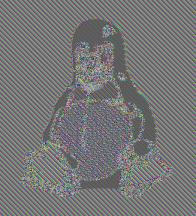
\includegraphics[width=\textwidth]{images/Tux_ecb.jpg}
		\caption{ECB-Modus}
	\end{subfigure}
	\hfill
	\begin{subfigure}[b]{.3\textwidth}
		\centering
		
\includegraphics[width=\textwidth]{images/Tux_secure.jpg}
		\caption{anderer Modus, z.B. CTR}
	\end{subfigure}
	\flushright{\scriptsize{Quelle: Larry Ewing, 1996 \cite{Ewing1996}}}
	\caption{Beispielhafter Vergleich verschiedener Modi}
	\label{fig:tux_encryption_modes}
\end{figure}

Fundamentale Eigenschaften der einzelnen Modi sind in der unteren Tabelle aufgeführt. Beachte, dass die hier vorgestellten Modi nur ein Teil einer Vielzahl an existierenden Betriebsmodi sind.
\begin{table}[h]
	\captionsetup{labelformat=empty}
	\captionsetup{singlelinecheck=false}
	\captionsetup{font=footnotesize}
	\centering
	\begin{tabularx}{\textwidth}{ | >{\raggedright\arraybackslash}X | >{\raggedright\arraybackslash}X | >{\raggedright\arraybackslash}X | >{\raggedright\arraybackslash}X | >{\raggedright\arraybackslash}X |} 
		\hline
		& ECB & CBC & CTR & GCM\\ 
		\hline
		Hauptsächliche Verwendung & Nachrichten, die kürzer als ein Block sind & Nachrichten, die länger als ein Block sind
		& Nachrichten, die länger als ein Block sind & Nachrichten, die länger als ein Block sind und vor Manipulationen geschützt werden müssen\\ 
		\hline
		\parbox{3cm}{IND-CPA\(^{\ast}\) } sicher & Nein & Ja$^{\ast\ast}$ & Ja$^{\ast\ast}$ & Ja$^{\ast\ast}$\\
		\hline
		 Parallelisierbar & Ja & Nur Entschlüsselung  & Ja & Ja, das Signieren selbst aber nicht\\ 
		\hline
		Bit-Fehler im Block $\ciphert_i$ an Stelle $j$ & Block $\plaint_i$ zerstört & Block $\plaint_i$ zerstört und Bit $j$ im Block $\plaint_{i+1}$ negiert 
		& Bit $j$ im Block $\plaint_i$ negiert & Bit $j$ im Block $\plaint_i$ negiert und geänderte Signatur\\
		\hline
	\end{tabularx}
	\caption{$^{\ast}$ IND-CPA ist ein Sicherheitsbegriff und wird in \hyperref[def:ind-cpa]{Abschnitt \ref{def:ind-cpa}} definiert\\ 
		$^{\ast\ast}$ Hierfür muss der $IV$ vor jeder Verschlüsselung zufällig gleichverteilt gewählt werden}
\end{table}
